% outline.tex -- writer's outline (8-page article). Build: tectonic outline.tex  (natbib plainnat, refs.bib)
\documentclass[10pt]{article}
\usepackage[margin=1.7cm]{geometry}
\usepackage{amsmath,amssymb}
\usepackage{enumitem}
\usepackage{multicol}
\usepackage[authoryear,round]{natbib}
\usepackage{url}
\usepackage{graphicx,booktabs,array}
\usepackage{changes}% tracked edits; use \usepackage[final]{changes} for clean text
\definechangesauthor[name={Pass 3}, color=teal]{P3}
\usepackage{todonotes}
\usepackage[hidelinks]{hyperref}
\setlist{nosep,leftmargin=1.2em,topsep=0pt,itemsep=0pt}
\setlength{\emergencystretch}{3em}
\setlength{\parindent}{0pt}
\setlength{\parskip}{0pt}
\renewcommand{\bibfont}{\scriptsize}
\setlength{\bibsep}{0pt}
\newcommand{\pp}[2]{\par\vspace{3pt}\noindent\textbf{#1.}\ #2\par\nopagebreak}
\newcommand{\res}[1]{[\textit{result: #1}]}
\newcommand{\tbd}[1]{[\textit{to be decided: #1}]}
\newcommand{\hd}[2]{\section*{#1 \hfill {\normalfont\small #2}}\vspace{-4pt}}

\begin{document}
\begin{center}
{\large\bfseries \replaced{Benchmarking alignment penalties for single-cell batch correction}{Wasserstein critics versus discriminators for single-cell batch correction}}\\[2pt]
{\small Kendall Reid$^{1,*}$, Genevieve Stein-O'Brien$^{2,\dagger}$, Erhan Guven$^{3,\dagger}$}\\[1pt]
{\footnotesize $^1$Department of Computer Science, Johns Hopkins University; $^2$Department of Neuroscience, Johns Hopkins University; $^3$Johns Hopkins University Applied Physics Laboratory. $^*$Corresponding author\added[id=P3]{: kreid20@jh.edu}. $^\dagger$These authors contributed equally.}\\[1pt]
{\footnotesize \deleted[id=P3]{Keywords: single-cell RNA sequencing; batch correction; adversarial learning; optimal transport; benchmarking}}
\end{center}
{\footnotesize \textbf{Writer's outline.} \replaced[id=P3]{Target: \emph{BMC Bioinformatics}, Research article; structured abstract at most 350 words; 3 to 10 keywords; no stated word, figure or reference limit; Declarations required; large language model use documented in Methods.}{Target: \emph{Bioinformatics Advances}, Original Article, 8 pages; abstract at most 200 words; at most 6 figures, 6 tables, 50 references; no citations in the supplement.} Main text about 5,000 words plus 400 words of captions; paragraphs 100--150 words. Brackets: fill from results or still open. \replaced[id=P3]{Background}{Introduction} and Methods are the first author's prose with tracked corrections (\texttt{changes} package; change logs in \texttt{paper/drafts\_20261022/}). Figures 1--6 and Tables 3--4 are mocks; \replaced{Table 1 holds real design facts and Table 2 provisional pilot ranges, to be replaced when the all-task pilot is scored}{Tables 1--2 hold real design facts}.}

\hd{Abstract}{\replaced[id=P3]{at most 350 words; Background, Results, Conclusions}{200 words; 7 sentences}}
\begin{enumerate}[leftmargin=1.5em]
\item \added[id=P3]{\textbf{Background:}} \replaced{Batch correction for single-cell data often adds an alignment penalty (an adversarial discriminator, a Wasserstein-1 critic estimating the earth mover's distance, or a direct distance between batches) to a deep generative model, but penalties have rarely been compared on one backbone.}{Adversarial batch correction trains an encoder against a discriminator predicting each cell's batch; a Wasserstein-1 (W1) critic, estimating the earth mover's distance between batches, is an alternative.}
\item \replaced{Question: which alignment penalty keeps the most biology at equal batch removal in one scVI (single-cell variational inference) model, and does any beat plain scVI or standard tools at equal tuning effort?}{Question: does swapping the Jensen--Shannon (JS) discriminator for a W1 critic change biology kept at equal batch removal in scVI (single-cell variational inference)?}
\item \replaced{Benchmark on eight tasks of the single-cell integration benchmark: scVI plus the Jensen--Shannon discriminator, three Wasserstein-1 critics (reference, pooled, barycenter), maximum mean discrepancy or the Sinkhorn divergence, with the decoder given the batch label or not.}{Pre-registered comparison, eight tasks of the single-cell integration benchmark (scIB): scVI plus JS discriminator, three W1 critics (reference, pooled, barycenter), maximum mean discrepancy (MMD) or Sinkhorn divergence; decoder with or without batch label.}
\item \added[id=P3]{\textbf{Results:}} \replaced{\res{ranking of the six penalties by biology at matched batch removal: mean rank over the real tasks that are not low-signal, per decoder, simulations reported separately.}}{[result: biology at matched batch removal, reference critic minus discriminator, per decoder.]}
\item \replaced{\res{trade-off area, collapse rate, local versus global removal, good-strength range and label transfer per penalty.}}{[result: trade-off area, collapse rate, local versus global removal, good-strength range.]}
\item \replaced{\res{placement against plain scVI, Harmony, Scanorama, sysVI, scANVI at equal tries, including whether any penalty beats plain scVI.}}{[result: divergence versus regularisation and update steps; placement against plain scVI, Harmony, Scanorama, sysVI, scANVI at equal tries, including whether any adversary beats plain scVI.]}
\item \added[id=P3]{\textbf{Conclusions:}} \res{one-sentence guidance for scVI users.} Code and checksums: \tbd{repository address and version tag at submission}.
\end{enumerate}
\par\vspace{3pt}\noindent\added[id=P3]{\textbf{Keywords:} single-cell RNA sequencing; batch correction; adversarial learning; optimal transport; benchmarking}

\section[Background]{\replaced[id=P3]{Background}{Introduction}}
% intro_tracked.tex -- Introduction of USER_DRAFT with tracked corrections.
% Markup: LaTeX `changes' package (\added{new}, \deleted{old}, \replaced{new}{old}).
% Preamble needed by the integrating document:  \usepackage[authoryear,round]{natbib}  \usepackage{changes}
%   (build with \usepackage[final]{changes} to print the corrected text only).
% \protect precedes \citep inside \deleted{} so that the strike-out markup does not break the citation.
% Change log with sources: intro_changelog.md. Bibliography: paper/refs.bib (no new entries needed).
% Base text: brief/user_draft.tex lines 42-54 (Introduction), checked against paper/outline.tex Intro-1..8 (commit 8c89960).

\qquad Single-cell RNA-seq experiments provide a snapshot of a cell's transcriptional activity at a point in time; however, the biological differences in a dataset can be overshadowed by technical differences between experimental samples. Laboratory conditions, reagent lots, personnel and instruments introduce technical variation, which becomes a confounder when it is correlated with the biological outcome \citep{leek2010tackling,yu2024assessing}. In single-cell RNA-seq, separately processed technical replicates can differ substantially \citep{tung2017batch}, and single-cell data bring new challenges for modelling batch effects \citep{goh2022batch}. This has led to a variety of batch correction methods, among them Harmony \citep{korsunsky2019fast}, Scanorama \citep{hie2019efficient}, scVI (single-cell variational inference) \citep{lopez2018deep}, its label-aware extension scANVI \citep{xu2021probabilistic} and sysVI \citep{hrovatin2025integrating}. A central challenge of these methods is to balance the alignment of batches with the preservation of biological signal \citep{luecken2022benchmarking}. Under-correction results in datasets that retain substantial batch effects, while over-correction discards key biological information \citep{yu2024assessing}.

\qquad With the adoption of deep learning-based methods in single-cell analysis, techniques for trainable end-to-end batch correction are necessary. A notable class of deep-learning approaches, latent-variable models, aim to learn a low-dimensional representation of the RNA-seq readout that captures salient signals corresponding to biological programs. To align these latent spaces across batches, two primary methods have been adopted: decoder conditioning, which passes the batch label as an input variable to the decoder responsible for reconstructing the input RNA-seq vector from the latent variable \citep{lopez2018deep}, and adversarial batch, which trains a network to predict the batch, or another confounder such as age, from each cell's latent code and penalizes the encoder whenever that prediction succeeds  \citep{ganin2016domain,dincer2020adversarial}.

\qquad Adversarial methods are split between discriminator approaches, which minimize the Jensen--Shannon (JS) divergence \citep{goodfellow2014generative} between samples from different batches or confounding variables \citep{ganin2016domain,dincer2020adversarial}, and Wasserstein critic-based methods, which minimize the Wasserstein-1 (W1) distance \citep{arjovsky2017wasserstein,gulrajani2017improved} between such samples. These techniques have been applied extensively to single-cell batch correction.

\qquad iMAP trained a critic with the gradient penalty of the Wasserstein generative adversarial network (WGAN-GP), correcting every dataset towards one anchor dataset that is left unchanged \citep{wang2021imap}. iDLC trains a WGAN-GP critic, with a Sinkhorn transport term added to the generator loss, to map each source batch onto a reference batch \citep{jiang2026geometric}; scStarCorrect also aligns every batch to one fixed reference batch, but through a domain-aware discriminator whose loss form its abstract does not state \citep{gu2025scstarcorrect}; Beaconet trains one Wasserstein critic per batch against the mixture of the other batches and needs no reference \citep{xu2024beaconet}. IMGG trains a WGAN-GP generator towards a synthetic intermediate batch built from cells matched across batches \citep{wang2022imgg}, ResPAN combines a Wasserstein GAN with random-walk mutual-nearest-neighbour pairing \citep{wang2022respan}, and IMAAE uses a loss of WGAN-GP form, an anchor batch and known cell labels \citep{wang2023integrating}. Methods built on a standard discriminator are numerous as well. Portal trains two logistic discriminators and clamps their logits so that cells scored as clearly dataset-specific give no gradient and are not forced to mix \citep{zhao2022adversarial}; AIF pairs a real-versus-reconstructed discriminator with a batch classifier that the encoder is trained against \citep{monnier2024novel}; and ABC trains an autoencoder against a multi-class batch discriminator alongside cell-type classifier branches that use labels \citep{danino2024batch}.

\qquad A third route avoids training an adversary network altogether by measuring the distance between the latent batches explicitly. These include the maximum mean discrepancy (MMD) \citep{gretton2012kernel}, and optimal transport (OT) measures \citep{cuturi2013sinkhorn, genevay2018learning,feydy2019interpolating}. A full mathematical formulation of these approaches is available in \replaced{Supplementary Note 1}{supplementary note XXX}. Both measures have been used to align single-cell batches without an adversary. MMD-ResNet trains a residual network to match the distribution of one batch to that of another \citep{shaham2017removal}, SAUCIE applies an MMD penalty against a reference batch on an internal layer \citep{amodio2019exploring}, trVAE places an MMD term across conditions in the first decoder layer \citep{lotfollahi2020conditional}, uniPort couples a variational autoencoder with minibatch unbalanced OT \citep{cao2022unified}, and Li et al.\ added an MMD term between batches to the loss of an early scVI version \citep{li2022trade}.

\qquad Despite their promise, \replaced{alignment penalties}{adversarial methods} have limitations that challenge their utility in practice. When batches contain different cell-type proportions, a lower bound on classification error grows as the latent distributions of the two batches are aligned more tightly \citep{zhao2019learning}, and exact alignment under any divergence that is zero only for identical distributions leaves an error at least as large as the proportion gap \citep{wu2019domain}. The sysVI study found that an adversarial conditional variational autoencoder and an adversarial multi-omics integration method mixed unrelated cell types when proportions were unbalanced across batches, and more so at higher adversarial strength \citep{hrovatin2025integrating}; dataset imbalance also changed clustering, annotation, differential expression, query mapping and trajectories across five integration methods \citep{maan2024characterizing}.

% This section below should be a short sentence of two before the result

% \added{Image-GAN studies caution against attributing a difference to the divergence alone. With enough hyperparameter search and random restarts, most GAN losses reached similar scores, and none consistently beat the original non-saturating loss \citep{lucic2018gans}; that loss was stable across datasets, spectral normalisation helped consistently, and the gradient penalty helped only sometimes \citep{kurach2019large}. A difference between a critic and a discriminator may therefore come from regularisation, the number of adversary updates or tuning rather than from the divergence. These are image results; our follow-up experiment tests whether they carry over, by varying the regulariser and the update steps while holding the backbone fixed.}


\replaced{\qquad Batch-correction methods have been compared in several large benchmarks \citep{tran2020benchmark,luecken2022benchmarking,luecken2025defining}. These benchmarks compare complete methods, each with its own architecture, preprocessing and training settings, so they cannot show which alignment objective accounts for a method's performance. Controlled comparisons of alignment losses inside one framework are few.}{\qquad Controlled comparisons of alignment losses exist, but none covers the critic.} \replaced[id=P3]{The extended single-cell integration benchmark (scIB-E)}{scIB-E} compared six batch losses, one of them a GAN discriminator, inside one scVI framework, with no Wasserstein, MMD or OT term \citep{yi2025benchmarking}; Li et al.\ compared MMD with an adversarially trained mutual-information penalty on an early scVI version and traced the Pareto front between batch removal and biology \citep{li2022trade}; and the iDLC ablation removes its Sinkhorn term but has no JS or MMD arm \citep{jiang2026geometric}. In searches of OpenAlex, arXiv and Europe PMC run in October 2026, we found no study that compares JS, W1 and MMD or OT objectives on one stock scVI backbone. This absence is search-based, not exhaustive \tbd{repeat the literature search before submission}.

\deleted{\qquad Batch-correction methods have been compared in several large benchmarks (\mbox{\citealt{tran2020benchmark}}; \mbox{\citealt{luecken2022benchmarking}}; \mbox{\citealt{luecken2025defining}}). These benchmarks compare complete methods, each with its own architecture, preprocessing and training settings, so they cannot show which alignment objective accounts for a method's performance. The one benchmark that compared batch losses inside a single scVI framework included a discriminator, but no Wasserstein, MMD or optimal-transport objective (\mbox{\citealt{yi2025benchmarking}}).}

\qquad In this study we benchmark discriminator-, critic-, kernel- and optimal transport-based alignment penalties for batch correction. We compare the JS discriminator, three variants of the Wasserstein critic (reference, pooled and barycenter), MMD and the Sinkhorn divergence with standard baselines. Each penalty is added to the same scVI model \citep{lopez2018deep}, with the decoder either given the batch label or not, and evaluated on eight tasks of the single-cell integration benchmark scIB \citep{luecken2022benchmarking}. \replaced{The backbone and tasks are fixed, and the training settings are fixed except the adversary update steps and optimiser, which follow each method's usual setting, so differences between methods come from the alignment penalty as it is usually run.}{The backbone, training settings and tasks are fixed, so differences between methods come from the alignment penalty alone.}

% this should be in methods
% We compare all of these approaches with plain scVI and with Harmony \citep{korsunsky2019fast}, Scanorama \citep{hie2019efficient}, scANVI \citep{xu2021probabilistic} and sysVI \citep{hrovatin2025integrating} at equal numbers of tries, allowing for the outcome that no alignment penalty improves on plain scVI.
% A stronger penalty trades biology for batch removal along a curve, as Li et al.\ showed for scVI \citep{li2022trade}. We therefore read each method's biology score where all methods reach the same batch removal. For each penalty we also report how often it collapses and how narrow its range of good strengths is.
% DONE: moved to Methods (matched-batch-removal, baselines and secondary-analysis paragraphs)


\section{Methods}
% methods_tracked.tex -- Methods of USER_DRAFT with tracked corrections (LaTeX `changes` package:
% \added{}, \deleted{}, \replaced{new}{old}). Preamble needs \usepackage{changes} and the \tbd macro of outline.tex.
% Change numbers (C1, C2, ...) refer to methods_changelog.md. \todo commands of the draft are removed; their text is
% shown as \deleted{\textit{todo: ...}} so the deletion is visible.
% Written 2026-10-21 from the sources listed in methods_changelog.md. No main-benchmark or follow-up result was read.

% ---- Paragraph 1: backbone (user paragraph 1) ----
\qquad To establish a fair comparison between methods, we use a fixed backbone from the well-established scVI (single-cell variational inference) architecture \citep{lopez2018deep}, implemented in the scvi-tools python package \citep{gayoso2022python}. Every method uses scvi-tools' default settings and likelihood with epochs, minibatch size and latent size equal within a task, so that the alignment method and its strength are the only intended differences\added{, apart from the adversary update steps and their optimiser, which follow each method's usual setting (Supplementary Note 2)}. We apply this across two scenarios: a conditioned setting in which the batch label is fed to the decoder, as scVI is usually run, and an unconditioned setting in which no batch label reaches the encoder or decoder, so the adversary is the only correction\added{ (Figure 1a)}. The full hyperparameter and training details are available in Supplementary Table S2 and Supplementary Note 2.

% This should be in supplement
% DONE: moved to Supplementary Note 2
% Two differences are by design: the discriminator takes one update step per training step with the generator's optimiser settings, whereas the critics take five steps with their own Adam settings (learning rate $10^{-4}$, betas 0 and 0.9).
% (10 latent dimensions, one hidden layer of 128 units, a zero-inflated negative binomial likelihood; Supplementary Table S2 and Supplementary Note 2),
% Plain scVI is the same model at strength zero. The adversary reads the encoder's posterior mean without per-dimension standardisation, two defaults kept after pre-registered pilots (Supplementary Note 2), and every fit is scored on the posterior mean.

% ---- Paragraph 2: penalties (user paragraph 2) ----

% This should be in supplement each trained with a gradient penalty of weight 10
% DONE: moved to Supplementary Note 1

\qquad Each method adds a fixed penalty, weighted by a fixed strength, to the normal scVI loss (Table 1). The discriminator predicts each cell's batch and the encoder minimizes scvi-tools' bounded fool loss, a Jensen--Shannon (JS) type objective \citep{goodfellow2014generative}. We test three Wasserstein-1 (W1) critic-based methods\citep{arjovsky2017wasserstein}, \citep{gulrajani2017improved}: reference based, pooled, and barycenter. The reference method aims to align all batches with a single reference batch, which we assign based on the highest cell-type entropy \todo{we need justification here}.\added{ A reference that contains every cell type gives each batch a target for all of its cell types, so no batch is pushed onto cell types the reference lacks \tbd{confirm this justification}.} The pooled critic compares each batch against the cells of all other batches pooled together. The Wasserstein barycenter approach \citep{cuturi2014fast} estimates an average distribution of the batches present in each minibatch, recomputed at every step, and aligns every batch to it. The network-free approaches are the maximum mean discrepancy (MMD) of each batch to the others, with a fixed multi-scale Gaussian kernel \citep{gretton2012kernel}, and the debiased Sinkhorn divergence, an entropy-regularised optimal transport (OT) distance \citep{cuturi2013sinkhorn,genevay2018learning,feydy2019interpolating}, which at the smoothing used is not an estimate of W1. For the full details of the loss equations and the training settings, see Supplementary Notes 1 and 2.

% This level of detail should be in the supplement
% DONE: moved to Supplementary Note 3
% fit on its posterior-mean embedding, on all cells, with scIB's metrics unscaled, and summarise them as

% ---- Paragraph 3: data and metrics (user paragraph 3) ----
\qquad We benchmark these methods on eight integration tasks of the single-cell integration benchmark (scIB) \citep{luecken2022benchmarking}, used as distributed with their batch and cell-type labels. These consist of six real datasets from different biological settings, four of single-cell RNA sequencing (human pancreas, lung, immune cells, and joint human--mouse immune cells) and two of chromatin accessibility (\added{assay for transposase-accessible chromatin, }ATAC; mouse brain, a small and a large dataset, as gene-activity matrices), and two simulated datasets. RNA tasks use 2,000 highly variable genes and the ATAC tasks all features; counts are used as distributed. The full details of the datasets are available in Supplementary Table S1. We score each method using the scIB batch, biology, and aggregate selection scores. The batch score is the mean of five metrics: principal-component regression on batch, batch average silhouette width (ASW), graph integration local inverse Simpson's index (iLISI), graph connectivity and the k-nearest-neighbor batch-effect test (kBET). The biology score is the mean of the task's biology metrics: normalized mutual information and adjusted Rand index between clusters and cell-type labels, cell-type ASW, isolated-label F1, isolated-label silhouette, graph cell-type LISI (cLISI), plus cell-cycle conservation on the four real RNA tasks and trajectory conservation on the two immune tasks, which have pseudotime. The mathematical formulation of these metrics is available in Supplementary Note 3. The scIB combined selection score is the weighted average $0.4\,\mathrm{batch} + 0.6\,\mathrm{biology}$\added{.}

% ---- Paragraph 4: strength pilot (user paragraph 4) ----
\qquad To identify the range of adversarial strengths tested for each penalty family, we run a pilot study fitting plain scVI and the six penalties at ten strengths\replaced{ in half-decade steps from 0.1 to 3,000}{ (0.1, 0.3, 1, 3, 10, 30, 100, 300, 1,000 and 3,000)} on all datasets across three seeds\added[id=P3]{, with two further edge strengths in two places: 0.01 and 0.03 for the discriminator with the unconditioned decoder, and 10,000 and 30,000 for the Sinkhorn divergence with the conditioned decoder}. One range is set per penalty family and decoder, the three critics sharing one because their strength multiplies the same quantity: eight ranges. Using seed means, each range runs from the largest strength at which no pilot task differs from plain scVI (no failed fit, batch and biology scores within noise) to the smallest strength from which every task has stopped gaining batch removal or has collapsed (a failed fit, or biology 0.10 or more below plain scVI); six strengths are spread evenly on a log scale over it, and where that span holds fewer than six half-decade values, neighbouring values are added, above first. In the cases where the response reaches the edge of the grid, the grid is extended by the next two half-decade values beyond that edge and the rule re-run\replaced{; \tbd{number of extended ranges and their values, from the all-task pilot}}{; this happened twice (36 extra fits), for the discriminator with the unconditioned decoder (0.03 and 0.01) and for the Sinkhorn divergence with the conditioned decoder (10,000 and 30,000)}. The resulting ranges are displayed in Table 2\added{ \tbd{final ranges and the six strengths per family and decoder, from the all-task pilot; Table 2 shows provisional values}}. The full details on how these ranges were chosen are available in Supplementary Note 4.

% This should be in the supplement
% DONE: moved to Supplementary Note 11 (run counts) and Table S5
% (480 fits each), 3,000 fits in all; a fit fails if its training loss or its latent becomes non-finite}{5 seeds}.

% ---- Paragraph 5: main benchmark and matched batch removal (user paragraph 5) ----
\qquad To benchmark the performance of each penalty, we fit it at the six strengths of its family on all eight tasks. We fit both conditional and unconditional decoders across five seeds: plain scVI and the six penalties. Because strength has a different scale for each penalty and \replaced{a stronger penalty trades biology for batch removal along a curve, as Li et al.\ showed for scVI \citep{li2022trade}}{biology trades off against batch removal}, we do not compare methods at a fixed strength. Instead we identify, for each task and decoder, a batch score, $b^*$, halfway between plain scVI's mean batch score and the highest mean batch score that every one of the six penalties reaches (Supplementary Note 5)\added{; we therefore read each penalty's biology score at $b^*$, a batch removal that every penalty reaches (Figure 1b)}. This matched level only works if the penalties remove clearly more batch effect than plain scVI. We call a task and decoder pair low-signal when that gap is under 0.02, so that $b^*$ sits less than 0.01 above plain scVI\replaced{ and cannot be placed reliably}{, below the smallest difference we count as real}; low-signal pairs are left out of the \replaced{ranking}{comparisons made at $b^*$}, shown in a separate table\deleted{ and never pooled}. \replaced{The pilot identifies which pairs are low-signal: \tbd{low-signal task--decoder pairs, from the all-task pilot}.}{In the pilot two pairs were low-signal, both with the conditioned decoder: immune (gap 0.019) and simulation 1 (gap 0.007).}

% % ---- New paragraph (a): statistical analysis (from Meth-7, Meth-9, Meth-11; PREREG, SPEC) ----
% This section is too focused on the critic vs discriminator, it needs to be generalized to the new benchmark.
% \added{\qquad The primary comparison is the reference critic's biology score at $b^*$ minus the discriminator's, per task and decoder, read by linear interpolation on each method's curve of seed-mean scores from plain scVI through its six strengths, with uncertainty from repeating the reading with each seed left out (Supplementary Note 5 gives the rules for when a task is evaluable). The six real tasks are pooled in one model that weights each task by its uncertainty and lets related tasks share a family effect, because the human--mouse immune task contains all immune cells and the large chromatin-accessibility task contains all cells of the small one; the priors have scale 0.1, the model is integrated exactly, and simulations are reported per task and never pooled. We declare a direction if the posterior probability that the overall difference lies beyond a margin of 0.01 on one side is at least 0.95, practical equivalence if the probability that it lies within $\pm0.01$ is at least 0.95, and otherwise the result is inconclusive \citep{corani2017statistical}. The six primary results (this comparison, the trade-off area and the collapse rate, each per decoder) are judged on their own posteriors; an exact Wilcoxon signed-rank test with Holm's correction over the six is reported as description only, because with six tasks its smallest attainable $p$, 0.031, exceeds the first threshold of $0.05/6$. From the pilot, the minimal detectable effect at 80\% power is 0.131 over the six real tasks, so the design is underpowered. The pilot rules were frozen on 4 October 2026, their amendments and this analysis on 16 October 2026, before anyone had read a main-benchmark score, and the analysis runs once (Supplementary Note 11).}

\added{\qquad The main analysis is a descriptive ranking. For each task and decoder, a penalty's curve joins plain scVI and its six strengths by seed-mean scores, and its biology score is read at $b^*$ by linear interpolation where the curve first reaches $b^*$ (Figure 1b). For each penalty, task and decoder the uncertainty is the standard error of that reading over repeats with each of the five seeds left out in turn, holding $b^*$ fixed and leaving the same seed out of plain scVI, and the range (lowest to highest) of the penalty's rank over the five repeats. These are reported only if at least four of the five leave-one-seed-out readings exist, and otherwise as not available; the penalty is ranked either way (Supplementary Note 5). A task and decoder pair is ranked unless it is low-signal. Within each ranked pair the six penalties are ordered by biology at $b^*$ (rank 1 is best); tied penalties get the average of their ranks. A penalty whose curve does not reach $b^*$ takes the bottom rank in that pair, penalties that all fail sharing the last places, following scIB, where methods that could not be run on a task were given the same rank as unintegrated data \citep{luecken2022benchmarking}. As in scIB, the mean rank over all real tasks that are not low-signal is reported for each decoder; simulations are ranked and reported separately, and low-signal pairs are shown separately and left out of the ranking (Supplementary Note 6). We report no significance tests: ranks and their uncertainty describe the data. Each penalty's selection score is also compared with plain scVI's, at one strength not tuned on the task and as the expected best of $k$ tries (below). The pilot and analysis rules were fixed before any main-benchmark score was read \tbd{confirm once the analysis plan and code carry the ranking rules} (Supplementary Note 10).}

% ---- New paragraph (b): baselines (from Meth-2, Meth-13; paper.tex 436-447; SPEC section 9) ----
\qquad We place the penalties against plain scVI and against standard tools: scvi-tools' own adversarial classifier (its built-in batch classifier, run with the conditioned decoder only), Harmony \citep{korsunsky2019fast}, Scanorama \citep{hie2019efficient}, sysVI \citep{hrovatin2025integrating}, scANVI, which uses the cell-type labels \citep{xu2021probabilistic}, and principal-component analysis (PCA) as the uncorrected reference.\added{ We compare all of these approaches at equal numbers of tries, allowing for the outcome that no alignment penalty improves on plain scVI.}\added{ Harmony, Scanorama and sysVI run at six settings each}\deleted{ (Harmony's diversity penalty from 0 to 8 at 10 principal components, Scanorama's neighbour count from 2 to 80 at 10 dimensions, sysVI's cycle-consistency weight from 1 to 50)}\added{, scANVI and PCA at one}\deleted{; the neural tools use seeds 0--4 and the others one run, 408 fits including three sensitivity settings (Harmony at 50 principal components, Scanorama at 100 dimensions and PCA at 50 components; Supplementary Table S4 and Supplementary Note 8)}\added{ (settings, seeds and fit counts in Supplementary Table S4 and Supplementary Note 8). A try is one setting of a method, fitted and scored.} \added{Because the penalties and the tools have different numbers of settings, placement compares methods at equal numbers of tries, by the expected best selection score among $k$ settings drawn at random, and is descriptive.}\added{ Each penalty is also scored at one strength not tuned on that task, the strength with the best mean selection score on the real tasks of the other task families, shown beside the task's own best strength as an optimistic bound (Supplementary Note 7).}\added[id=P3]{ Harmony, Scanorama and sysVI get their setting by the same rule: the setting with the best mean selection score on the real tasks of the other families, with the task's own best setting in parentheses as the optimistic bound (Supplementary Note 8). scANVI and PCA run at one setting, so they involve no choice.}

% ---- New paragraph (c): follow-up experiment (from Meth-14 to Meth-16; PREREG 721-790; SPEC-FU) ----

% This section is too focused on critic vs distriminator.
% DONE: dropped (first author's decision)
% \added{\qquad A follow-up experiment asks whether any critic--discriminator gap comes from the divergence itself or from the regularisation, optimiser and update steps that also differ between the two. On the small chromatin-accessibility, immune and pancreas tasks, with both decoders and three fresh seeds (10--12), it fits nine settings: the discriminator plain, with spectral normalisation \citep{miyato2018spectral}, with an R1 gradient penalty, a penalty on the discriminator's gradient at real data only \citep{mescheder2018training}, and with spectral normalisation plus the critics' Adam settings, each at one step; and the pooled critic with gradient penalty at 1, 5 and 10 steps and with spectral normalisation at 1 and 5 steps (Table 1, Supplementary Table S5). Each setting runs at three strengths, its base method's matched strength on the main benchmark (the strength whose batch score is nearest $b^*$) and the two grid neighbours, so the follow-up starts only after the main benchmark is scored: 486 fits. One contrast per decoder is confirmatory, the spectrally normalised pooled critic minus the spectrally normalised discriminator with the critics' optimiser, both at one step, which differ only in the loss and its target. Biology is read at $b^*$ where a setting's three strengths bracket it, pooled with the same model, margin and 0.95 rule, with Holm's correction over the two results; the divergence is said to explain the main gap only if the primary comparison and this contrast have a declared direction of the same sign and every regularisation and step-count contrast is smaller (Supplementary Note 9). Because both arms of this contrast inherit strengths chosen for other settings, a pre-check of 36 fits (18 per arm, on the pilot tasks at seed 100) decides by a rule fixed in advance whether each arm's three strengths move one half-decade step up, move down or stay: \tbd{pre-check outcome for each arm}.}

\added{\qquad For each penalty we also report how often it collapses and how narrow its range of good strengths is, together with its trade-off area, its local versus global batch removal and label transfer; all five views are descriptive, and each rule is given in full in Supplementary Note 7. A fit collapses if it fails or its biology score is at least 0.10 below the same seed's plain scVI; the collapse rate is the collapsed share of a penalty's fits in a task and decoder, with exact binomial (Clopper--Pearson) 95\% intervals \citep{clopper1934use}. The good-strength width is the span, in decades, of the strengths whose mean selection score is at least the lower 95\% confidence bound of the best strength's mean. The trade-off area is the part of the batch-score by biology-score plane that a penalty's six points reach beyond a corner at plain scVI's batch score and 0.10 below its biology score, divided by the batch gap that sets $b^*$ so that tasks share one scale.}

\added{\qquad Local removal is the mean of the three neighbourhood batch metrics (iLISI, kBET and graph connectivity) and global removal the mean of the two whole-embedding metrics (principal-component regression and batch ASW), so that at $b^*$ more local removal means less global; we report each penalty's local minus global reading at its crossing of $b^*$. Label transfer holds each batch out in turn and predicts its cell types from the other batches with a 15-nearest-neighbour classifier, on each penalty's embedding at the strength whose batch score is nearest $b^*$, never chosen by accuracy (Supplementary Note 9).}

\added[id=P3]{\qquad Large language model tools were used for writing and checking analysis code, running and checking computational jobs, and drafting and editing text. The authors checked all outputs and take responsibility for the content \tbd{first author to confirm tools, versions and roles}.}

\hd{Results}{1,500 words; \replaced{8}{10} paragraphs}
\pp{Res-1}{We first report which fits completed and where batch removal could be matched.}
\begin{itemize}
\item Rule: a fit fails when its loss or latent values become non-finite; failed fits are counted, and the matched batch-removal level $b^*$ uses only strengths with no failed fit (Supplementary Note 5, Table S\replaced{5}{6}).
\item \replaced{\res{fits completed and failed per method and decoder (counts in Supplementary Table S5).}}{[result: fits completed and failed per method and decoder, of 3,000 main fits (80 plain scVI, 40 scvi-tools adversarial classifier, 480 per penalty) plus 408 baseline fits.]}
\item \res{low-signal pairs (gap between plain scVI's batch score and the highest batch score every penalty reaches under 0.02, so $b^*$ cannot be told apart from plain scVI); methods never reaching $b^*$\added[id=P3]{ (ranked last in that pair)}.} \replaced{Low-signal pairs are left out of the ranking and shown in a separate table}{Low-signal readings go to a separate table and are never pooled} (Supplementary Note 5).
\end{itemize}
\pp{Res-2}{\replaced{Penalties are ranked by the biology they keep at matched batch removal (Figure 2, Table 3).}{The premise check reports how separable batches are before integration and how adversary gradients behave in training (Figure 2).}}
\begin{itemize}
\item \deleted{Rule: separability is the area under the receiver operating characteristic curve (AUC; 0.5 chance, 1 perfect) of a 15-nearest-neighbour batch classifier with five-fold cross-validation, run on the 80 plain-scVI embeddings (8 tasks, 2 decoders, 5 seeds) and averaged over batches; batches count as nearly separable when the AUC is at least 0.95 in all five seeds of a task and decoder (Supplementary Note 10).}
\item \deleted{Rule: the per-epoch logs of the 2,880 penalty fits give each adversary's gradient norm with respect to the embedding (before multiplying by strength) and, for the discriminator, its batch accuracy; a gradient vanishes early if it stays at or below 10\% of its own peak from within the first 10\% of epochs; no strengths or seeds are selected (Supplementary Note 10).}
\item \deleted{[result: separability per task (2a); gradient norm per epoch at preset strengths (2b); discriminator accuracy (2c).]}
\item \deleted{Exploratory, descriptive; no pooled test and no claim on whether the premise holds. Per-task detail in Supplementary Figure S3.}
\item \added{Rule: for each task and decoder, biology at $b^*$ is read where a penalty's curve first reaches $b^*$, interpolating between neighbouring strengths, with the standard error of the reading and the range of its rank over repeats with each of the five seeds left out; the six penalties are ranked by it (rank 1 is best; ties share the average rank; a penalty whose curve does not reach $b^*$ takes the bottom rank), and the mean rank over the real tasks that are not low-signal is reported per decoder (Methods; Supplementary Notes 5 and 6).}
\item \added{\res{mean rank per penalty and decoder with its range over tasks; how many real tasks each decoder's ranking rests on; which penalties are first or last in most tasks.}}
\item \added{\res{biology at $b^*$ per penalty, task and decoder with leave-one-seed-out standard errors and rank ranges (Supplementary Table S6); whether the readings of neighbouring ranks lie within one standard error of each other; low-signal pairs shown separately and pairs where a curve never reaches $b^*$ marked; simulations ranked per task (Supplementary Figure S1).}}
\item \added{Descriptive: no significance test or decision rule; sensitivity of the ranking to the reading rules in Supplementary Figure S2.}
\end{itemize}
\pp{Res-3}{Figure 3 shows each method's trade-off between batch removal and biology in every real task.}
\begin{itemize}
\item Rule: each method's curve joins plain scVI and its six strengths by their mean batch and biology scores over five seeds; the vertical line marks $b^*$ and the standard tools appear as points (Supplementary Note 5).
\item \res{curves: overlap, early ends, collapse.}
\item Simulations per task: Supplementary Figure S1. Per-metric curves: Supplementary Figure S\replaced{4}{5}.
\end{itemize}
\pp{\deleted{Res-4}}{\deleted{The primary comparison reports biology kept at matched batch removal, reference critic minus discriminator, for each decoder (Figure 4a, Table 3).}}
\begin{itemize}
\item \deleted{Rule: biology at $b^*$ is read where each curve first reaches $b^*$, interpolating between neighbouring strengths; uncertainty comes from repeating the reading with each of the five seeds left out; a task is not evaluable if it is low-signal, if either curve never reaches $b^*$, or if fewer than four of the five readings exist (Supplementary Note 5).}
\item \deleted{Rule: the six real tasks are pooled in the model of the Methods statistics paragraph; a direction is declared at posterior probability of at least 0.95 beyond the 0.01 margin, practical equivalence at 0.95 within $\pm0.01$, otherwise inconclusive (Supplementary Note 6).}
\item \deleted{[result: pooled estimate, 95\% interval, three posterior probabilities, call; each decoder.]}
\item \deleted{[result: per-task estimates; evaluable tasks; Wilcoxon companion (descriptive: Holm over the six primary results, first threshold $0.05/6=0.0083$, cannot reject with six tasks); simulations per task (Supplementary Figure S1).]}
\end{itemize}
\pp{\replaced{Res-4}{Res-5}}{\replaced{Trade-off area and collapse rate give two further views of each penalty (Figure 4a,b, Supplementary Table S8).}{Trade-off area and collapse rate give a second and third view of the same comparison (Figure 4b,c, Table 3).}}
\begin{itemize}
\item \replaced{Rule, trade-off area: as in Methods; low-signal pairs are left out (Supplementary Note 7).}{Rule, trade-off area: the area of the batch-score by biology-score plane that a method's six points reach beyond a corner at plain scVI's batch score and 0.10 below its biology score, divided by the batch gap that sets $b^*$; low-signal pairs are left out; reference critic minus discriminator, pooled as in Res-4 (Supplementary Note 7).}
\item \replaced{Rule, collapse: as in Methods; low-signal pairs are kept (Supplementary Note 7).}{Rule, collapse: a fit is collapsed if it fails or its biology score is at least 0.10 below the same seed's plain scVI; the collapse rate is the collapsed share of 30 fits per method, task and decoder, with exact binomial (Clopper--Pearson) 95\% intervals; the reference critic's rate minus the discriminator's is pooled with a margin of 5 percentage points, and low-signal pairs are kept (Supplementary Note 7).}
\item \replaced{\res{trade-off area per penalty, task and decoder; collapse rate with intervals per penalty, task and decoder; failure types.}}{[result: trade-off area difference; collapse rate with intervals, pooled difference, call; per decoder.]}
\item \deleted{[result: sensitivity to prior scale (0.05 and 0.2 against 0.1) and to dropping low-signal tasks (Supplementary Note 6, Supplementary Figure S2).]}
\end{itemize}
\pp{\replaced{Res-5}{Res-6}}{\replaced{We then report whether each penalty removes batch effects more locally or more globally, and the label-transfer check (Figure 4c\added{; label transfer in Supplementary Figure S3}).}{We then report whether batch removal is more local with a critic, and the label-transfer check (Figure 4d).}}
\begin{itemize}
\item \replaced{Rule, local versus global: the batch score is $(3\,\mathrm{local}+2\,\mathrm{global})/5$, so at $b^*$ more local removal means less global; each penalty's local-minus-global reading is taken at the crossing of its biology reading and reported without a test (Methods; Supplementary Note 7).}{Rule, local versus global: local removal is the mean of three neighbourhood metrics (integration local inverse Simpson's index, k-nearest-neighbour batch-effect test, graph connectivity) and global removal the mean of two whole-embedding metrics (principal-component regression, batch average silhouette width); the batch score is $(3\,\mathrm{local}+2\,\mathrm{global})/5$, so at $b^*$ more local removal means less global. The reference critic's local-minus-global reading minus the discriminator's is taken at the primary comparison's crossing and tested with an exact sign test over real tasks and with the pooled model (Supplementary Note 7).}
\item \replaced{\res{local-minus-global reading per penalty, task and decoder; which penalties remove batch effects more locally.}}{[result: local-minus-global difference per decoder, sign test, pooled call.]}
\item \replaced{Rule, label transfer: matched strengths are chosen by batch score, never by accuracy; plain scVI and the scvi-tools adversarial classifier are labelled unmatched; the gap between the matched batch score and $b^*$ is printed beside each value; no test or decision rule; low-signal pairs are tabulated but left out of summaries (Methods; Supplementary Note 9, Supplementary Figure S3).}{Rule, label transfer: each batch is held out in turn and a 15-nearest-neighbour classifier trained on the other batches predicts its cell types, on each method's embedding at its matched strength (batch score nearest $b^*$, never chosen by accuracy) for five seeds, with plain scVI and the scvi-tools adversarial classifier labelled unmatched; cell types found in one batch only are dropped; F1 is computed per cell type and averaged, with the gap between the matched batch score and $b^*$ printed beside it; no test or decision rule; low-signal pairs tabulated but left out of summaries (Supplementary Note 10, Supplementary Figure S4).}
\item \res{label-transfer F1 per type (supplement), \replaced{descriptive}{exploratory}.}
\end{itemize}
\pp{\replaced{Res-6}{Res-7}}{The range of good penalty strengths is reported for every method (Figure 5\deleted{a}).}
\begin{itemize}
\item Rule: quality is the selection score (0.4 batch plus 0.6 biology); for each method, task and decoder the best strength has the highest mean selection score over five seeds, the good range holds every strength of the six (Table 2, Supplementary Table S3) whose mean is at least the lower end of the best strength's 95\% confidence interval, and the width is the span from smallest to largest good strength in decades; descriptive, no decision rule (Supplementary Note 7).
\item \res{width in decades per method, task, decoder; best strength at grid edge; no good range.}
\end{itemize}
\pp{\deleted{Res-8}}{\deleted{The regularisation and update-step follow-up reports whether a critic--discriminator difference comes from the divergence (Figure 5b).}}
\begin{itemize}
\item \deleted{Rule, read-out at matched strength: each follow-up variant runs at its base method's matched strength from the main benchmark (batch score nearest $b^*$) and its two grid neighbours; biology at $b^*$ is interpolated along the three strengths where they bracket $b^*$, with all three leave-one-seed-out readings required, otherwise the task is not evaluable; for every task the difference at the matched strengths is also reported, labelled fixed-strength (Supplementary Note 9).}
\item \deleted{Rule, confirmatory contrast and explanation: per decoder, the spectrally normalised pooled critic minus the spectrally normalised discriminator with the critic's optimiser, both at one step; 0.01 margin and 0.95 rule as in Res-4; Holm's correction over its two results (companion test cannot reject with three tasks, smallest $p$ 0.25); the divergence is said to explain the main gap only if Res-4 has a declared direction for that decoder, this contrast has the same direction, and every regularisation and step-count contrast is smaller in size; no direction with fewer than three evaluable tasks; failure counts replace collapse rates because the follow-up has no plain-scVI fits (Supplementary Note 9).}
\item \deleted{[result: biology at matched strength minus plain discriminator, per variant and decoder; confirmatory contrast: estimate, interval, call.]}
\item \deleted{[result: one, five, ten critic steps, pooled critic.]}
\end{itemize}
\pp{\replaced{Res-7}{Res-9}}{Single-strength tables place each method against plain scVI and the standard tools (Table 4, Figure 6b).}
\begin{itemize}
\item Rule: \replaced[id=P3]{each penalty, and each of Harmony, Scanorama and sysVI at one of its settings, is shown at a strength or setting not tuned on that task}{each penalty is shown at a strength not tuned on that task}, the one with the best mean selection score on real tasks of other families (related tasks never choose for each other), beside the task's own best strength as an optimistic bound\deleted{; Harmony, Scanorama and sysVI are run at six settings each, scANVI (uses cell-type labels) and PCA (uncorrected reference) at one, five seeds for the neural methods}; descriptive (Supplementary Notes 7 and 8, Table S4).
\item \res{selection score per method, decoder, task at strength from other families\added{, with its difference from plain scVI}; own-best strength as optimistic bound; batch against biology score per real task.}
\end{itemize}
\pp{\replaced{Res-8}{Res-10}}{The comparison at equal numbers of tries reports whether any \replaced{penalty}{adversary} improves on plain scVI (Figure 6a\added[id=P3]{; per-task curves in Supplementary Figure S6}).}
\begin{itemize}
\item Rule: each method gets the expected best selection score among $k$ of its settings drawn at random, $k=1$--6, so methods with more settings gain no advantage; optimistic because the best setting is chosen and scored on the same data; scANVI has its own stratum (Supplementary Note 7).
\item \res{expected best selection score at $k=1$--6 per family and decoder\added[id=P3]{ (Figure 6a shows the mean over the six real tasks of each method's per-task curve)}; whether any \replaced{penalty}{adversary} exceeds plain scVI, Harmony, Scanorama or sysVI.}
\item Descriptive; best-of-$k$ labelled optimistic.
\end{itemize}

\hd{Discussion}{700 words; 5 paragraphs}
\pp{Disc-1}{\replaced{\res{one-sentence answer to the main question for each decoder: which penalties rank highest by mean rank, and how close neighbouring ranks are.}}{[result: one-sentence answer to the main question for each decoder.]}}
\begin{itemize}
\item \replaced{\res{ranking at matched batch removal, trade-off area and collapse rate together; whether the order holds across tasks; what local-versus-global adds.}}{[result: primary comparison, trade-off area, collapse rate together; differences versus 0.01 margin; what local-versus-global adds.]}
\end{itemize}
\pp{Disc-2}{\replaced{\res{what the secondary analyses say about why penalties differ.}}{[result: what the follow-up and the premise check say about why methods differ.]}}
\begin{itemize}
\item \replaced{\res{whether the ranking is tight, as image-GAN losses were once each was tuned equally} \citep{lucic2018gans}.}{[result: divergence versus regularisation versus update steps], against image-GAN findings (\mbox{\citealt{lucic2018gans}}; \mbox{\citealt{kurach2019large}}).}
\item \deleted{[result: premise check] against theory (\mbox{\citealt{arjovsky2017towards}}); exploratory.}
\item Composition shift: tie over-correction to batch removal at matched level \citep{zhao2019learning,hrovatin2025integrating}.
\end{itemize}
\pp{Disc-3}{\replaced{\res{guidance for scVI users, including the outcome that no alignment penalty improves on plain scVI.}}{[result: guidance for scVI users, including the outcome that no adversary improves on plain scVI.]}}
\begin{itemize}
\item \res{when a penalty is worth adding; strength range; whether a standard tool does better at equal tries.} Word from placement results only.
\end{itemize}
\pp{Disc-4}{The design limits what the data can show.}
\begin{itemize}
\item \deleted{Underpowered (minimal detectable effect 0.131, six real tasks, 80\% power); Wilcoxon descriptive.} \replaced{Six real tasks in four families, two of them nested pairs (human--mouse immune contains all immune cells; large ATAC contains small); related tasks count as separate tasks in the mean rank, and the ranking is descriptive.}{Four families, two nested pairs (human--mouse immune contains all immune cells; large ATAC contains small).}\added[id=P3]{ A penalty whose curve does not reach $b^*$ is ranked last in that pair, so a missing reading counts as the worst result.}
\item \replaced{\tbd{strength grids set on the eight tasks of the all-task pilot; say what the pilot showed.} Regularisation (gradient penalty, spectral normalisation) and the number of adversary update steps were not varied: the reference, pooled and barycenter critics take five steps per encoder step and the discriminator one, so a difference between penalties includes these settings and is not due to the divergence alone.}{Strength grids set on three of eight tasks. Reference critic five steps, discriminator one; update-step control only for pooled critic.}
\item One batch variable per task; ATAC as gene-activity matrices; non-integer counts as distributed; scoring includes training cells; Sinkhorn not W1; reference choice uses labels.
\item \added[id=P3]{The collapse-rate intervals treat a penalty's 30 fits in a task and decoder as independent, although each seed's six fits are judged against the same plain-scVI threshold; in a simulation of the design their coverage was 0.91 to 1.00 for a nominal 0.95.}
\end{itemize}
\pp{Disc-5}{Several factors are outside the scope of this comparison.}
\begin{itemize}
\item Not varied or tested: architecture, \replaced{Kullback--Leibler (KL)}{KL} warm-up (incomplete on shorter tasks, penalty from start), reference batch, batch number; composition shift read from strength curves, not a dose-response test. Adversary steps reuse one minibatch.
\end{itemize}

\hd{\added[id=P3]{Conclusions}}{\added[id=P3]{about 150 words; 1 paragraph}}
\begin{itemize}
\item \added[id=P3]{\res{main conclusion: which penalties keep the most biology at matched batch removal, and whether any beats plain scVI or a standard tool at equal tries.}}
\item \added[id=P3]{\res{why it matters for scVI users: when a penalty is worth adding and at what strength.}}
\end{itemize}

\hd{\replaced[id=P3]{Declarations}{Availability and declarations}}{\replaced[id=P3]{eight BMC subheadings, each filled or marked not applicable}{50 words; 1 paragraph}}
\pp{\added[id=P3]{Ethics approval and consent to participate}}{\added[id=P3]{Only publicly available, previously published data are analysed (the tasks of the single-cell integration benchmark). \tbd{confirm wording}}}
\pp{\added[id=P3]{Consent for publication}}{\added[id=P3]{Not applicable.}}
\pp{\replaced[id=P3]{Availability of data and materials}{Avail-1}}{Code and data access.}
\begin{itemize}
\item Repository github.com/kreid415/wasserstein-critic-deconfounding; \tbd{version tag and commit at submission}; checksums in supplement.
\item \added[id=P3]{The eight task files are the integration-task datasets of the single-cell integration benchmark, figshare article 12420968, version 8 (doi:10.6084/m9.figshare.12420968.v8); file checksums in Supplementary Table S1.}
\item \deleted[id=P3]{Conflicts of interest: none declared; funding and author-contribution statements to be decided.}
\end{itemize}
\pp{\added[id=P3]{Competing interests}}{\added[id=P3]{\tbd{competing interests statement; the earlier outline said none declared, confirm with all authors}}}
\pp{\added[id=P3]{Funding}}{\added[id=P3]{\tbd{funding statement}}}
\pp{\added[id=P3]{Authors' contributions}}{\added[id=P3]{\tbd{authors' contributions statement}}}
\pp{\added[id=P3]{Acknowledgements}}{\added[id=P3]{\tbd{acknowledgements}}}
\pp{\added[id=P3]{Authors' information (optional)}}{\added[id=P3]{Not applicable.}}

\hd{Supplementary material}{\deleted[id=P3]{no citations; }Supplementary Notes 1--\replaced{11}{12}, Tables S1--S\replaced{8}{6}, Figures S1--S\replaced{6}{6}}
\textbf{Supplementary Notes}
\begin{itemize}
\item Supplementary Note 1, model and loss equations: scVI loss (zero-inflated negative binomial reconstruction, Kullback--Leibler (KL) term and KL weight schedule); discriminator fool loss as in scvi-tools (Jensen--Shannon type); the three Wasserstein-1 critics with gradient penalty weight 10: reference (each batch against the reference batch, chosen as the batch with the highest cell-type entropy, which uses labels), pooled (each batch against all others), barycenter (each batch against the minibatch Wasserstein barycenter, an average distribution); barycenter target construction\added{ and solver (Wasserstein-2, at most 10 iterations, threshold $10^{-7}$)}; maximum mean discrepancy (MMD) with multi-scale Gaussian kernel; debiased Sinkhorn divergence (entropy-regularised optimal transport; not W1 at the smoothing used\added{; Euclidean cost, entropic smoothing $0.05\sqrt{2d}$ for latent dimension $d$, float64, marginal error $10^{-4}$, cap of 500,000 iterations}); scvi-tools adversarial classifier (conditioned decoder only\added{; 32 hidden units, weight one minus the KL weight}); plain scVI as strength zero\added{; each critic head has two hidden layers of 128 units with one output per batch}.
\item Supplementary Note 2, training settings: \added{two differences between methods are by design, the update steps and the optimiser (both below; the discriminator uses the generator's optimiser settings); plain scVI is the same model at strength zero; zero-inflated negative binomial likelihood; } training split\added{ (90\%)}; minibatch\added{ (128)}; optimisers (critic optimiser: Adam, learning rate $10^{-4}$, betas 0 and 0.9\added{; generator and discriminator: Adam, learning rate $10^{-3}$, epsilon 0.01, weight decay $10^{-6}$}); update steps (one discriminator step, five critic steps per encoder step, by design; adversary steps reuse one minibatch); adversary input (posterior mean, no per-dimension standardisation) and \replaced{the two input pilots, whose switching criteria were fixed before they were run}{the two pre-registered input pilots} (two tasks, both decoders, three seeds: a posterior sample as input lowered biology at matched batch removal by mean $-0.004$, 9 of 12 task--decoder--method combinations evaluable, three adversarial methods; standardisation by $-0.003$, 14 of 20 evaluable, five methods; neither met the criteria for switching); scvi-tools epoch rule\added{ ($\min(400,\mathrm{round}(20000\times400/n))$ epochs for $n$ cells, no early stopping)} with epochs, minibatch and latent size equal within task; epochs and final KL weight per task; KL warm-up of 400 epochs, incomplete on four shorter tasks, so the penalty acts from step one; 10 latent dimensions, 128 hidden units; all scoring on the posterior mean; failed fit defined as non-finite loss or latent. Values in Table S2.
\item Supplementary Note 3, scIB metrics and scores: formulas of the five batch metrics (principal-component regression, batch average silhouette width, graph integration local inverse Simpson's index, graph connectivity, k-nearest-neighbour batch-effect test) and of each task's biology metrics, with the biology metric list per task; \added{each fit is scored on its posterior-mean embedding; }all metrics unscaled, raw 0--1, computed on all cells including training cells; batch score, biology score, selection score ($0.4$ batch $+ 0.6$ biology, the scIB overall weights); local (three neighbourhood metrics) and global (two whole-embedding metrics) split with batch score $(3\,\mathrm{local}+2\,\mathrm{global})/5$; input preparation: 2,000 highly variable genes, counts as distributed (non-integer in 18 batches of four tasks), chromatin-accessibility tasks as gene-activity matrices, one batch variable per task.
\item Supplementary Note 4, strength pilot: design (plain scVI and the six penalties at the ten half-decade strengths 0.1, 0.3, 1, 3, \replaced{10, 30, 100, 300, 1,000 and 3,000}{\ldots, 3,000} on \replaced{all eight tasks}{small chromatin-accessibility, immune and simulation 1 tasks}, both decoders, \replaced{seeds 100, 101 and 102, plus two edge strengths in two places (the discriminator with the unconditioned decoder also at 0.01 and 0.03, and the Sinkhorn divergence with the conditioned decoder also at 10,000 and 30,000); 378 fits per task (plain scVI 6; six penalties times ten strengths times three seeds times two decoders, 360; 12 edge-strength fits), 3,024 in all}{seeds 100--102, 1,098 fits}); the three-step choice rule on seed means (low end: largest strength at which no pilot task and method of the family differs from plain scVI, with no failed fit and both scores within noise; high end: smallest strength from which every task and method has stopped gaining batch removal or collapsed, a failed fit or biology 0.10 or more below plain scVI; six strengths spread evenly on a log scale, with neighbouring half-decade values added alternately above and below, starting above, when the range holds fewer than six); the noise threshold for no effect\added{ (the larger of 0.01 and three standard errors of the seed mean, using the median-unbiased seed standard deviation)}; edge extensions (two further strengths where a range reached the grid edge\replaced{; \tbd{ranges extended, extension values and number of fits, from the all-task pilot}}{, 36 fits, hence ranges ending at 0.03 and 10,000}); \replaced{\tbd{Sinkhorn pilot refit after the solver correction: confirm for the all-task pilot}}{Sinkhorn pilot refitted after a solver correction}; the chosen ranges (Table 2) and the six strengths per family and decoder (Table S3)\added{, both provisional until the all-task pilot is complete}; \replaced{\tbd{the low-signal pairs of the all-task pilot}}{the pilot's two low-signal pairs}.
\item Supplementary Note 5, matched batch removal and the low-signal rule: why equal strength is not equal correction; $b^*$ as the midpoint between plain scVI's mean batch score and the highest mean batch score all six penalties reach at strengths with no failed fit, per task and decoder\added{ (that highest score counts any edge-extension strengths of the main benchmark, while curves use only the six strengths, so a curve can fail to reach $b^*$)}; curve construction (plain scVI plus six strengths, seed means) and the interpolated reading where a curve first reaches $b^*$; \replaced[id=P3]{leave-one-seed-out standard error of the reading at fixed $b^*$ (the same seed left out of plain scVI) and range of the rank over the five repeats, reported only where at least four of five readings exist and otherwise as not available; which pairs are ranked (every pair that is not low-signal; a penalty whose curve does not reach $b^*$ takes the bottom rank)}{leave-one-seed-out uncertainty; evaluability (not low-signal, curve reaches $b^*$, at least four of five readings)}; the low-signal rule (gap under 0.02, so $b^*$ under 0.01 above plain scVI\replaced{ and not reliably placed}{, below the margin}) with the list of analyses that exclude low-signal pairs (\replaced{ranking at $b^*$}{biology at $b^*$}, trade-off area\added{, local versus global reading}) and keep them (collapse rate); the separate table of low-signal readings; \replaced{\tbd{pilot low-signal pairs and their values (plain scVI batch score, highest common batch score, gap), from the all-task pilot}}{pilot low-signal pairs (immune, conditioned decoder: plain scVI 0.638, highest common 0.657, gap 0.019; simulation 1, conditioned: 0.812, 0.819, gap 0.007)}; matched strength (batch score nearest $b^*$) as used by \deleted{the follow-up and }label transfer; failed-fit counting.
\item \replaced{Supplementary Note 6, benchmark ranking: how biology at $b^*$ is read for each penalty (curve of seed means through plain scVI and the six strengths, first crossing, linear interpolation), its leave-one-seed-out standard error (formula; $b^*$ held fixed, the same seed left out of plain scVI) and the range of its rank over the five repeats, reported only where at least four of five readings exist and otherwise as not available, the penalty being ranked either way; which pairs are ranked (every pair that is not low-signal); ranking rules (rank 1 is the highest biology at $b^*$ among the six penalties, ranks within each task and decoder; tied penalties get the average of their ranks, so two tied for 2nd both get 2.5, also for penalties sharing the bottom rank; a penalty whose curve does not reach $b^*$ takes the bottom rank in that pair and penalties that all fail share the last places, following scIB, where methods that could not be run on a task were given the same rank as unintegrated data \citep{luecken2022benchmarking}; mean rank over all real tasks that are not low-signal per decoder as in scIB, decoders never combined); simulations ranked and reported separately; low-signal pairs excluded from the ranking and shown in their own table; related tasks (human--mouse immune contains all immune cells; large chromatin-accessibility contains the small task) counted as separate tasks; sensitivity analyses of the reading (per-run reading, biology without trajectory conservation on the two immune tasks, points with a failed fit removed) and rank stability under the scaling checks (Supplementary Figures S2 and S5); no significance tests, probabilities, margins or multiplicity corrections.}{Supplementary Note 6, statistical analysis: the pooled model over the six real tasks (uncertainty weighting; family effect for four families: pancreas, lung, immune pair, chromatin-accessibility pair; nesting: human--mouse immune contains all immune cells, large chromatin-accessibility contains the small task); simulations and low-signal pairs never pooled; priors (scale 0.1; sensitivity 0.05 and 0.2); posterior probabilities and calls (direction at 0.95 beyond the margin, equivalence at 0.95 within the margin, otherwise inconclusive); margins (0.01 biology score; 5 percentage points collapse rate); multiplicity (descriptive Wilcoxon signed-rank with Holm's correction over the six primary results: comparison, area, collapse rate, per decoder; smallest attainable $p$ 0.031 exceeds $0.05/6=0.0083$); power from the pilot matched-strength contrast (minimal detectable effect at 80\% power 0.131 over six real tasks, 0.182 over four families; power 0.104 for a 0.02 difference; equivalence within $\pm0.02$ not showable); sensitivity analyses (prior scale, dropping low-signal tasks); the analysis is run once.}
\item Supplementary Note 7, rules for secondary analyses: trade-off area (corner at plain scVI's batch score and 0.10 below its biology, division by the batch gap, low-signal excluded, \replaced{reported per penalty, task and decoder}{pooled as the primary}); collapse (definition, \replaced{30 fits per penalty, task and decoder}{30 fits per cell}, exact binomial 95\% intervals, \deleted{pooled difference with 5 percentage point margin, }low-signal kept\added{, failure types reported separately}); local versus global (metric split, reading at \replaced{the same crossing as the biology reading, per penalty, descriptive}{the primary crossing, exact sign test over real tasks, pooled model}); good-strength width (selection score, best strength, window at the lower end of the best strength's 95\% confidence interval, width in decades, descriptive); single-strength placement (strength chosen on real tasks of other families, related tasks never choose for each other, \added{only strengths with no failed fit in any choosing task eligible, ties to the smaller strength, simulations take the strength chosen on all six real tasks, }own best as optimistic bound, descriptive\added[id=P3]{; the same rule picks the setting of Harmony, Scanorama and sysVI, Supplementary Note 8}); best-of-$k$ (expected best selection score among $k$ random settings, $k=1$--6, optimistic, scANVI in its own stratum, descriptive\added[id=P3]{; computed per task, with Figure 6a showing the mean over the six real tasks of each method's curve and the per-task curves in Supplementary Figure S6}\added{; plain scVI, scANVI and the scvi-tools adversarial classifier have one setting each, so plain scVI is the $k=1$ reference for each penalty's selection score}).
\item Supplementary Note 8, baselines: Harmony, Scanorama and sysVI at six settings each\added{ (Harmony's diversity penalty from 0 to 8 at 10 principal components, Scanorama's neighbour count from 2 to 80 at 10 dimensions, sysVI's cycle-consistency weight from 1 to 50)}; scANVI (uses cell-type labels) and principal-component analysis (uncorrected reference) at one setting\added[id=P3]{, so neither involves a choice; in the single-strength placement each of the three tools gets its setting by the same rule as the penalties (the setting with the best mean selection score on real tasks of other families, related tasks never choosing for each other, with the task's own best setting in parentheses as the optimistic bound)}; five seeds (0--4) for the neural methods, one run otherwise; 408 fits including \added{three }sensitivity settings\added{ (Harmony at 50 principal components, Scanorama at 100 dimensions, PCA at 50 components)}; grids and settings (Table S4); baseline grid amendments.
\item \deleted{Supplementary Note 9, follow-up experiment: design (small chromatin-accessibility, immune and pancreas tasks; both decoders; seeds 10--12; three strengths per setting, the base method's matched strength and its two grid neighbours; nine settings; 486 fits; run only after the main benchmark is scored); variants (discriminator at one step: plain, spectral normalisation, R1 gradient penalty, spectral normalisation plus the critic's optimiser; pooled critic with gradient penalty at 1, 5 and 10 steps and with spectral normalisation at 1 and 5 steps; pooled rather than reference critic) with the R1 weight, no gradient penalty on spectrally normalised critics, and the incomplete factorial design (Table S5); confirmatory contrast (spectrally normalised pooled critic minus spectrally normalised discriminator with the critic's optimiser, both one step); read-out rule (interpolation along the three strengths where they bracket $b^*$, all three leave-one-seed-out readings required, fixed-strength difference reported for every task); 0.01 margin and 0.95 rule; Holm's correction over two results (companion test cannot reject with three tasks, smallest $p$ 0.25); explanation rule and the requirement of at least three evaluable tasks for a direction; failure counts instead of collapse rates; the strength pre-check (36 fits, 18 per arm, small chromatin-accessibility, immune and simulation 1, both decoders, seed 100, at the three pilot strengths of the base method; reason: the discriminator arm's learning rate is ten times lower, the pooled-critic arm was never piloted; rule fixed before any pre-check fit: of the four non-low-signal pilot pairs, at least three below $b^*$ at all three strengths moves the arm one half-decade step up, at least three above moves it one step down, otherwise strengths stay; no second pre-check) and its outcome per arm once run.}
\item \replaced{Supplementary Note 9, label transfer: matched-strength embeddings for five seeds (the strength whose batch score is nearest $b^*$, never chosen by accuracy); plain scVI and the scvi-tools adversarial classifier unmatched; each batch held out in turn; 15-nearest-neighbour classifier; cell types in one batch only dropped, from labels alone; F1 per cell type averaged over types; gap to $b^*$ beside each value; low-signal pairs tabulated but not summarised; no test; the full label-transfer table.}{Supplementary Note 10, exploratory checks: premise check (80 plain-scVI embeddings; per-epoch logs of the 2,880 penalty fits; 15-nearest-neighbour batch classifier, five-fold cross-validation, AUC averaged over batches, nearly separable at 0.95 or more in all five seeds; gradient norm before multiplying by strength; discriminator accuracy; early-vanish rule, at or below 10\% of peak from within the first 10\% of epochs; no selection of strengths or seeds; descriptive) with per-task tables; label transfer (matched-strength embeddings for five seeds; plain scVI and the scvi-tools adversarial classifier unmatched; each batch held out in turn; 15-nearest-neighbour classifier; cell types in one batch only dropped, from labels alone; F1 per cell type averaged over types; gap to $b^*$ beside each value; low-signal pairs tabulated but not summarised; no test) with the full label-transfer table.}
\item \replaced{Supplementary Note 10, rules fixed before scoring and deviations: when the pilot rules and the ranking-analysis rules were fixed, and that no main-benchmark score had been read at that time \tbd{dates for the all-task pilot and the revised ranking analysis; confirm that no main-benchmark score was read before the ranking rules were fixed}; amendment list; early-scored fits (19 main-benchmark fits were scored and not read); grid-edge extension fits; post-pilot design choices (adversary input, standardisation, strength grids, matched strengths); baseline grid amendments; seed pairing; the ranking analysis run once, after all main fits are scored or failed; deviations from the plan fixed in advance; the long limitations list.}{Supplementary Note 11, registration and deviations: freeze dates (pilot rules 4 October 2026, before the pilot reported here; amendments and main-benchmark analysis 16 October 2026, before any main-benchmark score was read, 19 fits scored and unread; follow-up rule registered before any follow-up fit was scored); amendment list; early-scored fits; grid-edge extension fits; post-pilot design choices (adversary input, standardisation, strength grids, matched strengths); baseline grid amendments; seed pairing; the analysis run once; deviations from the registered plan; the long limitations list.}
\item Supplementary Note \replaced{11}{12}, software, hardware, run counts and checksums: scvi-tools and package versions; hardware; run counts per experiment (strength pilot \replaced{3,024 including 96 edge-strength fits (12 per task)}{1,098 plus 36 edge fits}; main benchmark 3,000\added{, made of 80 plain-scVI fits, 40 scvi-tools adversarial classifier fits and 480 fits per penalty (six strengths, two decoders, eight tasks, five seeds)}; baselines 408; \deleted{follow-up 486; pre-check 36; }input and standardisation pilots) with completed and failed fits (Table S\replaced{5}{6})\added{; a fit fails if its training loss or its latent becomes non-finite}; checksums of task files and results; repository and version tag. Scaling checks (Supplementary Figure S\replaced{5}{6}).
\end{itemize}
\textbf{Supplementary Tables}
\begin{itemize}
\item Table S1, tasks: for each of the eight tasks, cells, batches, cell types, genes (2,000 highly variable), real or simulated, family and nesting, count type as distributed (non-integer flag), gene-activity for chromatin-accessibility tasks, checksums.
\item Table S2, hyperparameters and training settings: latent dimensions (10), hidden units (128), likelihood (zero-inflated negative binomial), \added{training split (90\%), }minibatch, epochs per task from the scvi-tools rule, final KL weight per task, warm-up (400 epochs), optimisers, update steps, gradient penalty weight (10), adversary input, MMD kernel scales, Sinkhorn smoothing, seeds per experiment.
\item Table S3, strength ranges per penalty family and decoder: the no-effect end and the over-correction or collapse end of each chosen range, the six strengths of Table 2 with the neighbouring values added where the range held fewer than six marked, and edge extensions marked\added{; provisional values from the earlier three-task pilot, to be replaced by the all-task pilot}.
\item Table S4, baseline grids: the six settings of Harmony, Scanorama and sysVI, the single settings of scANVI and principal-component analysis, seeds, sensitivity settings.
\item \deleted{Table S5, follow-up variants: the nine settings with regulariser, update steps, optimiser, R1 weight, inherited strengths and pre-check adjustment.}
\item Table S\replaced{5}{6}, run counts: fits planned, completed and failed per experiment, method and decoder.
\item \added{Table S6, ranking detail: biology at $b^*$ per penalty, task and decoder with leave-one-seed-out standard errors, ranks and the range of each rank over the five repeats, a separate table of low-signal pairs, and the pairs where a penalty's curve does not reach $b^*$ marked.}
\item \added{Table S7, single-strength placement for the unconditioned decoder (the counterpart of Table 4): selection score per method and real task at the strength (for Harmony, Scanorama and sysVI, the setting) chosen on other task families, with the task's own best strength or setting in parentheses.}
\item \added{Table S8, secondary results per penalty, task and decoder: trade-off area, collapse rate with intervals and failure types, good-strength width and number of good strengths, local and global readings at $b^*$.}
\end{itemize}
\textbf{Supplementary Figures}
\begin{itemize}
\item Figure S1, simulation tasks: trade-off curves and per-task \replaced{ranking at $b^*$}{primary comparison}, each simulation on its own.
\item Figure S2, sensitivity: \replaced{ranking under alternative readings (per-run reading, biology without trajectory conservation on the two immune tasks, points with a failed fit removed).}{pooled estimates under prior scales 0.05, 0.1 and 0.2, and with low-signal tasks dropped.}
\item \deleted{Figure S3, premise-check detail: AUC per batch and task; gradient norm and discriminator accuracy per epoch at each strength.}
\item Figure S\replaced{3}{4}, label transfer: F1 per cell type, method and task at matched strength, with the gap to $b^*$.
\item Figure S\replaced{4}{5}, per-metric strength curves: each batch and biology metric against strength, per method and decoder.
\item Figure S\replaced{5}{6}, scaling checks.
\item \added[id=P3]{Figure S6, best of $k$ settings per task: each method's expected best selection score among $k$ settings drawn at random, $k=1$--6, one panel per real task; the mean of these curves over the six real tasks is Figure 6a.}
\end{itemize}

\hd{Figures and tables}{400 words of captions and notes}
\begin{itemize}
\item Figure 1: (a) model schematic: scVI encoder and decoder with or without the batch label, swappable alignment term; (b) how biology is read at matched batch removal $b^*$. Second cut, after Figure \replaced{5}{2}.
\item Figure 2: \replaced{ranking at matched batch removal: (a) heatmap of biology score at $b^*$ (colour) and rank (number) for the six penalties in each real task, conditioned and unconditioned decoder, not-ranked pairs hatched; (b) mean rank over the real tasks that are not low-signal per penalty and decoder with the range across tasks.}{premise check: (a) batch separability per task; (b) adversary gradient norm per epoch; (c) discriminator accuracy per epoch. First to move to the supplement if pages run short.}
\item Figure 3: biology score against batch score trade-off curves, decoders by real tasks, line per method, plain scVI point, $b^*$ line, standard tools as points.
\item Figure 4: \replaced{per-penalty dot plots, one point per real task and the mean: (a) trade-off area; (b) collapse rate with 95\% intervals; (c) local minus global batch removal at $b^*$.}{forest plots per task and pooled: (a) primary comparison; (b) trade-off area; (c) collapse-rate difference; (d) local minus global.}
\item Figure 5: \replaced{good-strength width per penalty and decoder, one point per task. First to move to the supplement if pages run short.}{(a) good-strength width per method; (b) follow-up variants minus plain discriminator.}
\item Figure 6: (a) expected best selection score against number of tries\added[id=P3]{, mean over the six real tasks of each method's per-task curve}; (b) batch against biology score at single strength.
\item Table 1: methods: alignment term, network, update steps, \replaced{strength grid family}{follow-up variants}.
\item Table 2: pilot strength ranges per penalty family and decoder (\replaced{provisional, from the earlier three-task pilot; to be replaced by the all-task pilot}{real pilot ranges}; cited by the Methods strength-pilot paragraph).
\item Table 3: \replaced{benchmark ranking: mean rank per penalty and decoder over the real tasks that are not low-signal, range over tasks, \added{mean biology at $b^*$, }simulation ranks, tasks not ranked, tasks ranked.}{primary results (primary comparison, trade-off area, collapse rate, per decoder): estimate, interval, probabilities, call, evaluable tasks.}
\item Table 4: single-strength placement: selection score per method, decoder, task.
\end{itemize}

\clearpage
% ---- Mock figures and tables (paper/drafts_20261022/figures_tables.tex; PNGs from make_mock_figures.py) ----
% figures_tables.tex -- mock figure and table environments for the paper outline.
% Requires: graphicx, booktabs, array, and the outline's \tbd{...} macro.
% PNGs: figures/mock/fig1.png ... fig6.png (MOCK watermark, synthetic data, 300 dpi, 17.4 cm wide).

% ---------------------------------------------------------------- Figure 1
\begin{figure}[t]
\centering
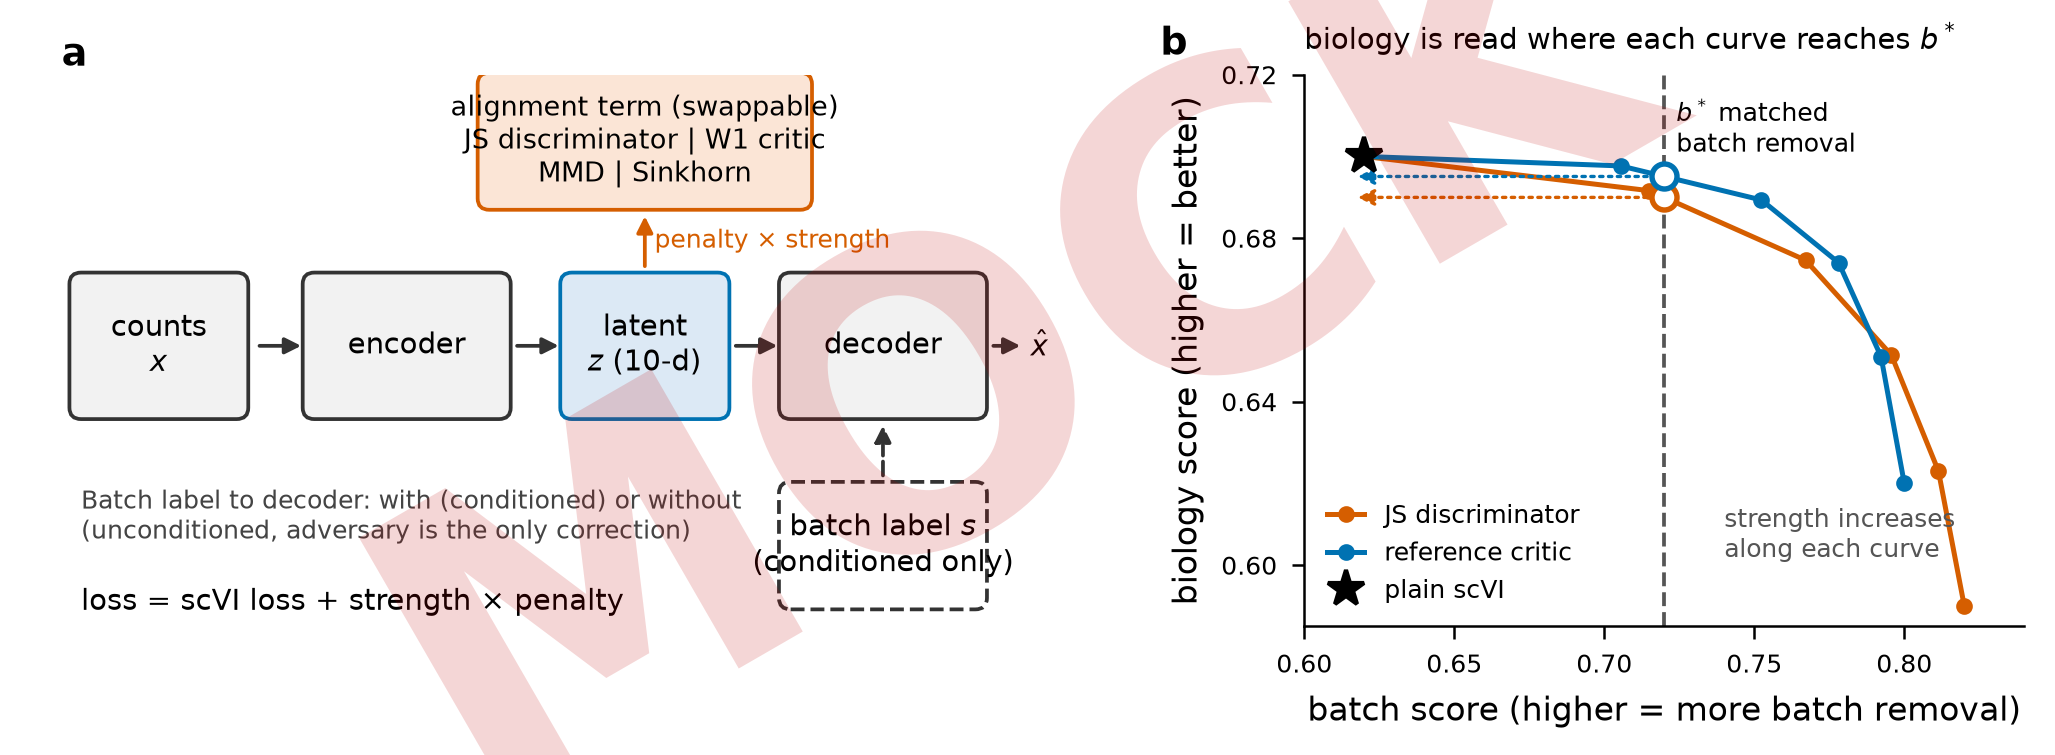
\includegraphics[width=\textwidth]{figures/mock/fig1.png}
\caption{MOCK -- synthetic data. Model and read-out. (a) One scVI encoder--decoder is shared by all methods; the decoder receives the batch label (conditioned) or not (unconditioned), and only the alignment penalty on the latent embedding is swapped. (b) Each strength curve joins plain scVI and six strengths; biology is read where the curve first reaches the matched batch removal $b^*$, interpolating between strengths. Placeholder schematic.}
\label{fig:1}
\end{figure}

% ---------------------------------------------------------------- Figure 2
\begin{figure}[t]
\centering
% MOCK NEEDS REDRAW: (a) heatmap of biology score at b* (colour) and rank (number) for six penalties by six real tasks, conditioned and unconditioned decoder, not-ranked (low-signal or unevaluable) cells hatched; (b) mean rank over the six real tasks per penalty and decoder with range across tasks. Replaces the old premise-check mock.
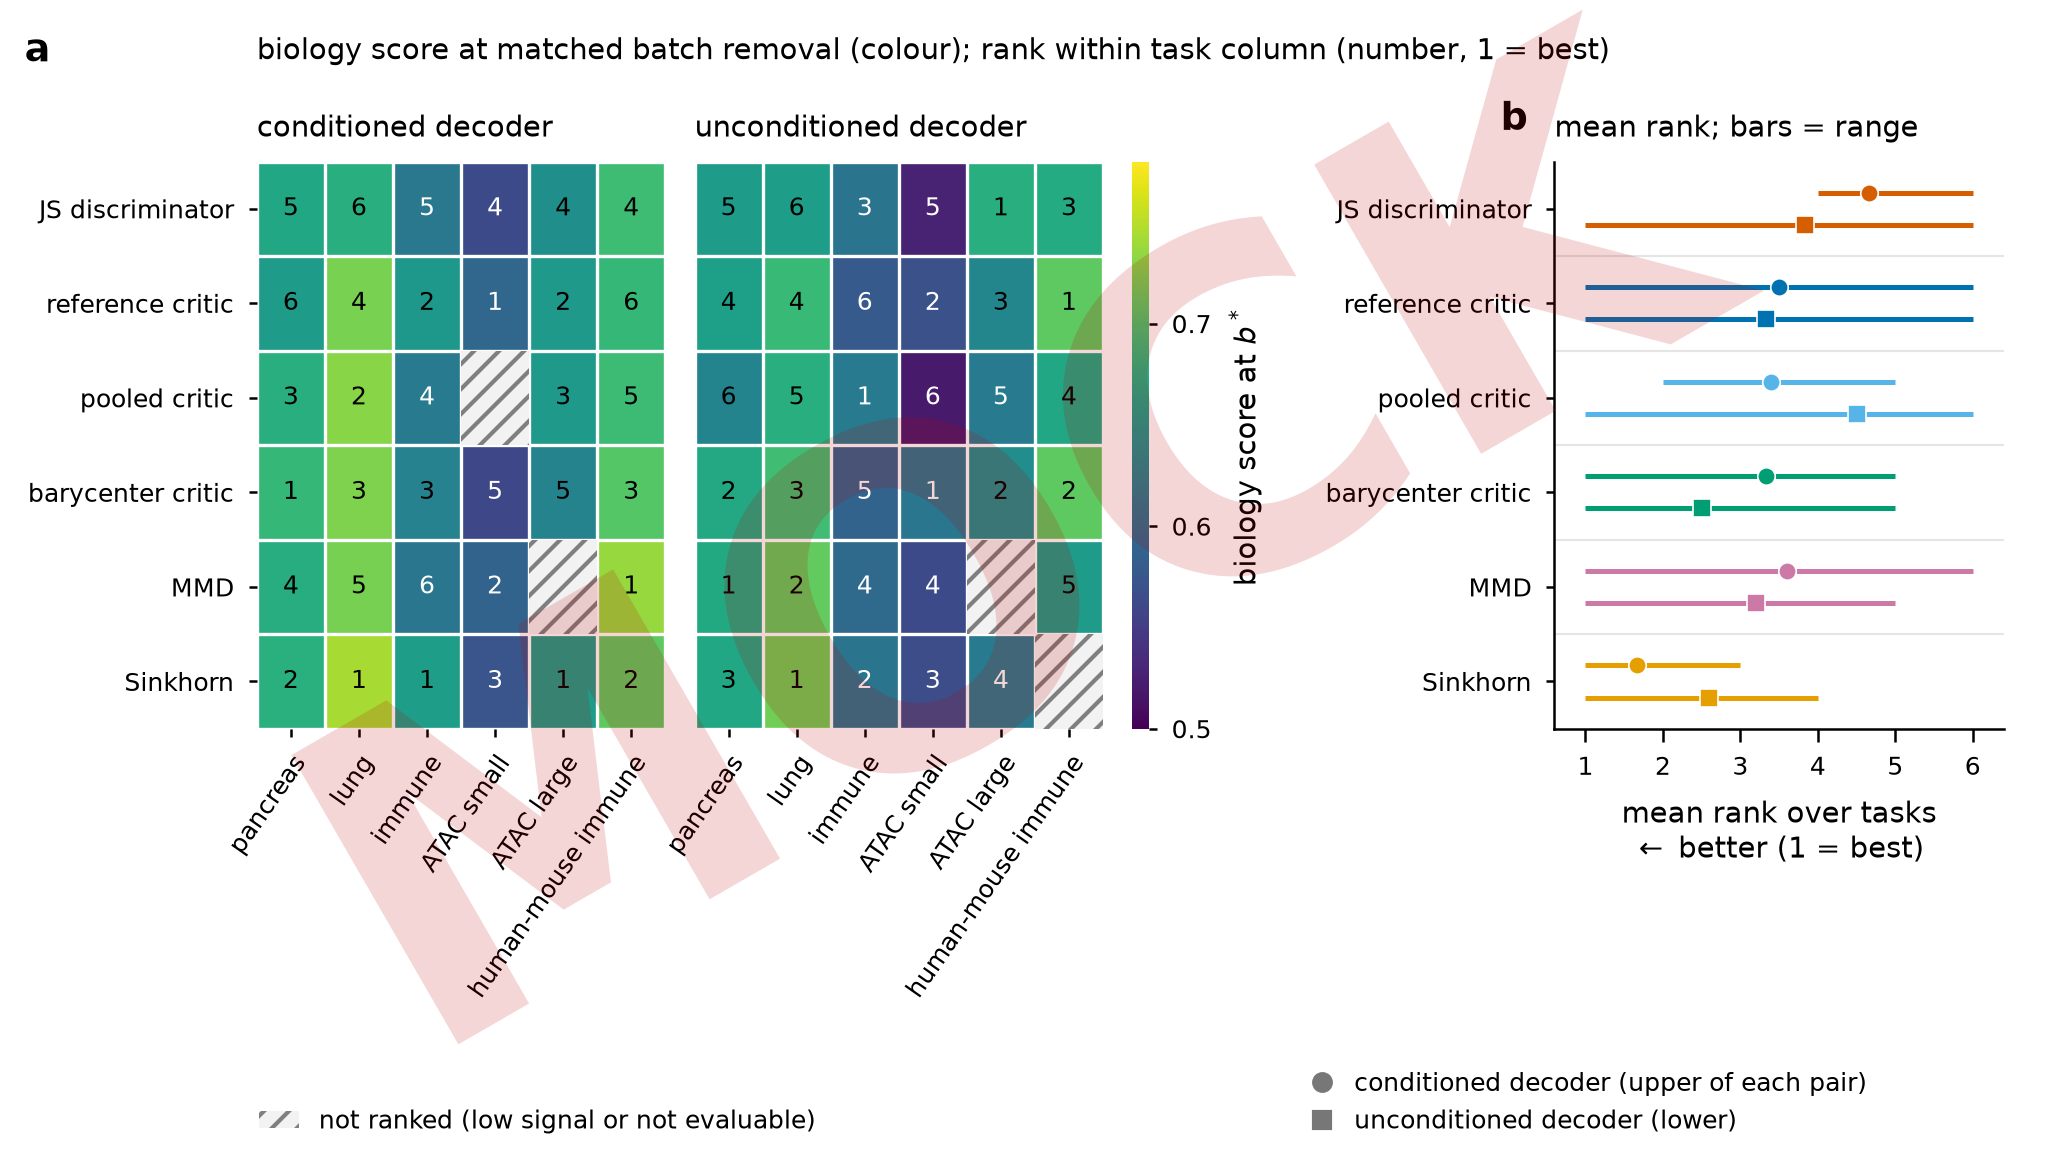
\includegraphics[width=\textwidth]{figures/mock/fig2.png}
\caption{\replaced{MOCK -- synthetic data. Ranking of the six penalties by biology kept at matched batch removal $b^*$. (a) Biology score at $b^*$ (colour) and rank within the column (number) for each real task, conditioned and unconditioned decoder; hatched cells are low-signal pairs and are not ranked; a penalty whose curve does not reach $b^*$ takes the bottom rank, and tied penalties share the average rank. (b) Mean rank over the real tasks that are not low-signal per penalty and decoder (rank 1 is best); bars, range over tasks. The leave-one-seed-out standard error of each reading in (a) and the range of each rank over the five leave-one-seed-out repeats are in Supplementary Table S6. Simulations are ranked separately (Supplementary Figure S1).}{MOCK -- synthetic data. Premise check (exploratory). (a) Batch separability of the plain-scVI embedding per task and decoder: area under the curve of a 15-nearest-neighbour batch classifier, one point per seed ($n=5$), tick is the mean, dashed line the 0.95 threshold. (b) Adversary gradient norm per epoch relative to its own peak, one line per penalty. (c) Discriminator batch accuracy per epoch, one line per task.}}
\label{fig:2}
\end{figure}

% ---------------------------------------------------------------- Figure 3
\begin{figure}[t]
\centering
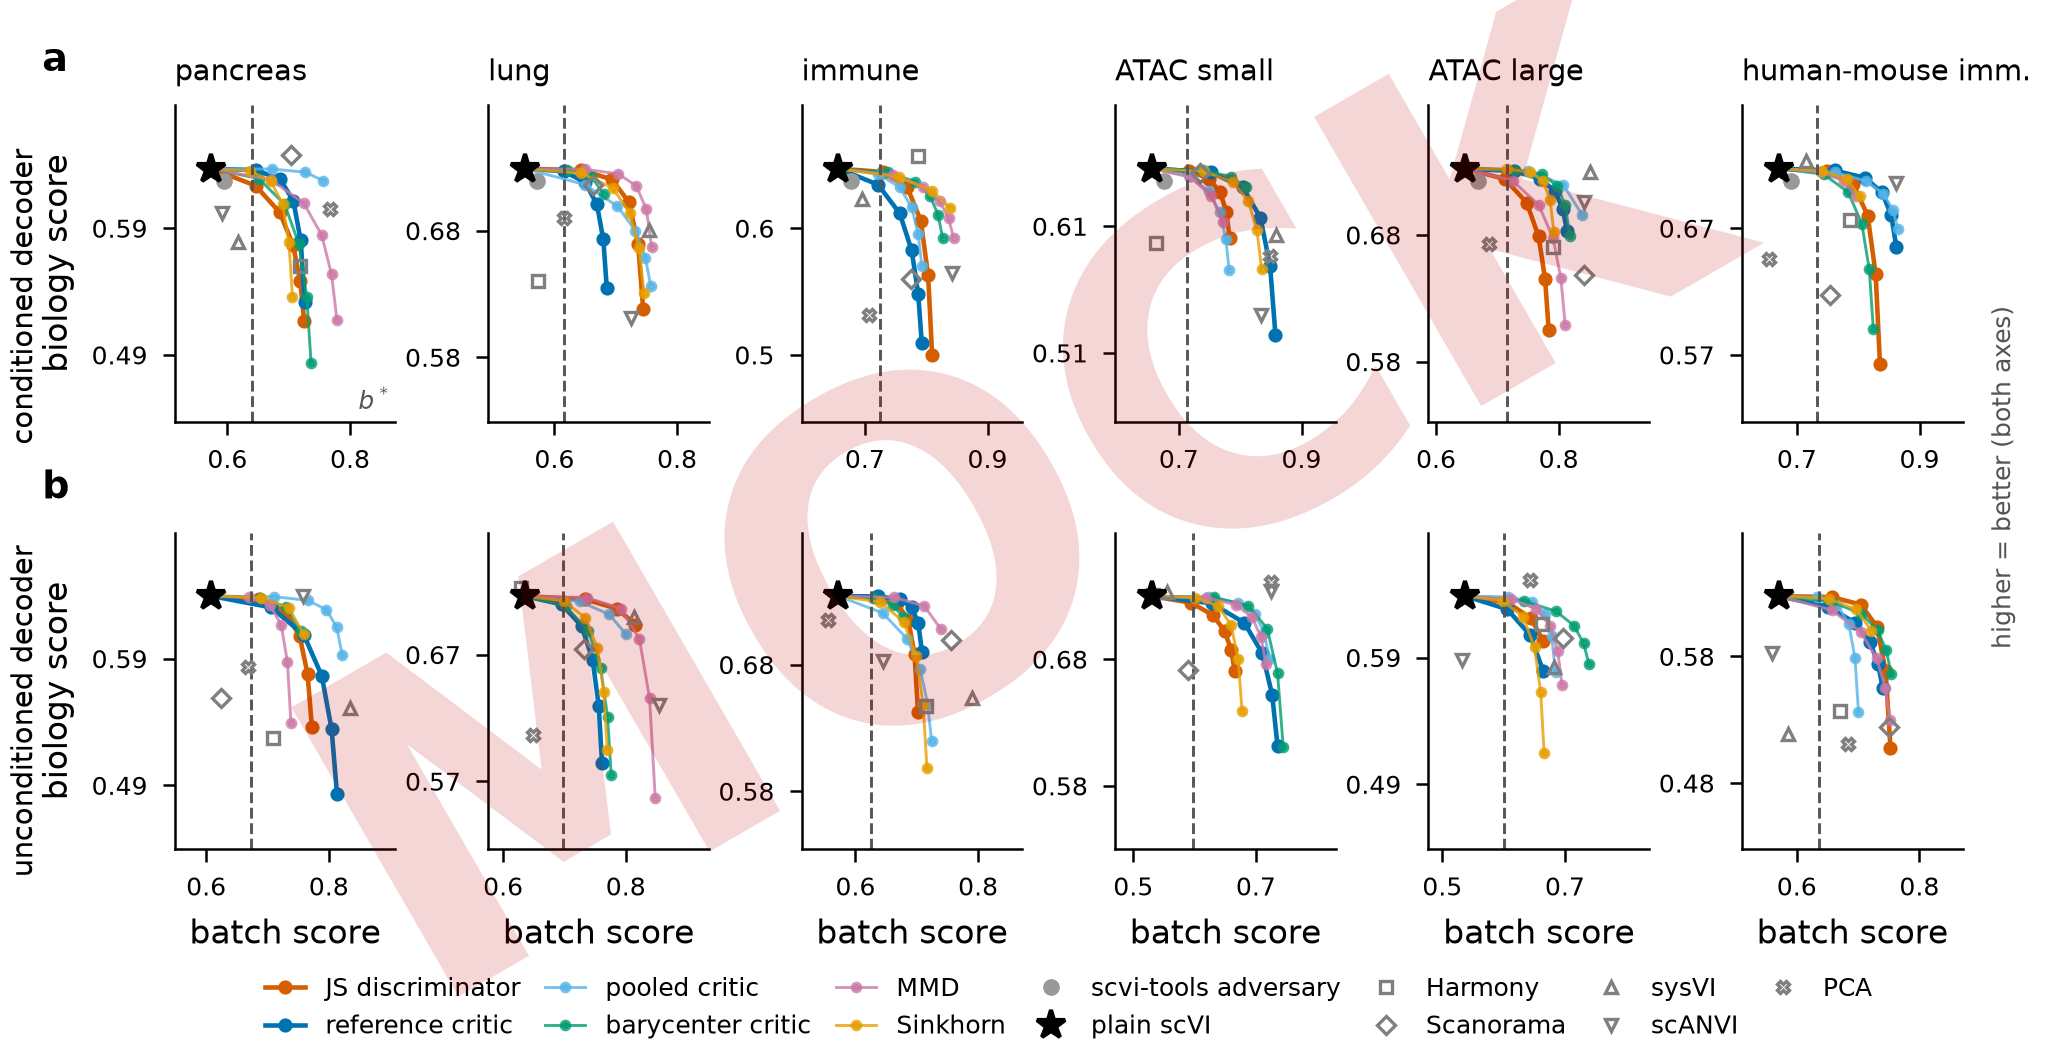
\includegraphics[width=\textwidth]{figures/mock/fig3.png}
\caption{MOCK -- synthetic data. Batch removal against biology kept in the six real tasks (columns) for the conditioned (a) and unconditioned (b) decoder. Each line joins plain scVI (star) and one penalty's six strengths by seed-mean scores (five seeds); a curve ending early marks collapsed fits. Dashed line, matched batch removal $b^*$. Grey open symbols, standard tools at their best setting.}
\label{fig:3}
\end{figure}

% ---------------------------------------------------------------- Figure 4
\begin{figure}[t]
\centering
% MOCK NEEDS REDRAW: per-penalty dot plots for the conditioned and unconditioned decoder, one point per real task plus the mean: (a) trade-off area; (b) collapse rate with exact 95% intervals; (c) local minus global batch removal at b*. Replaces the old reference-minus-discriminator forest plots.
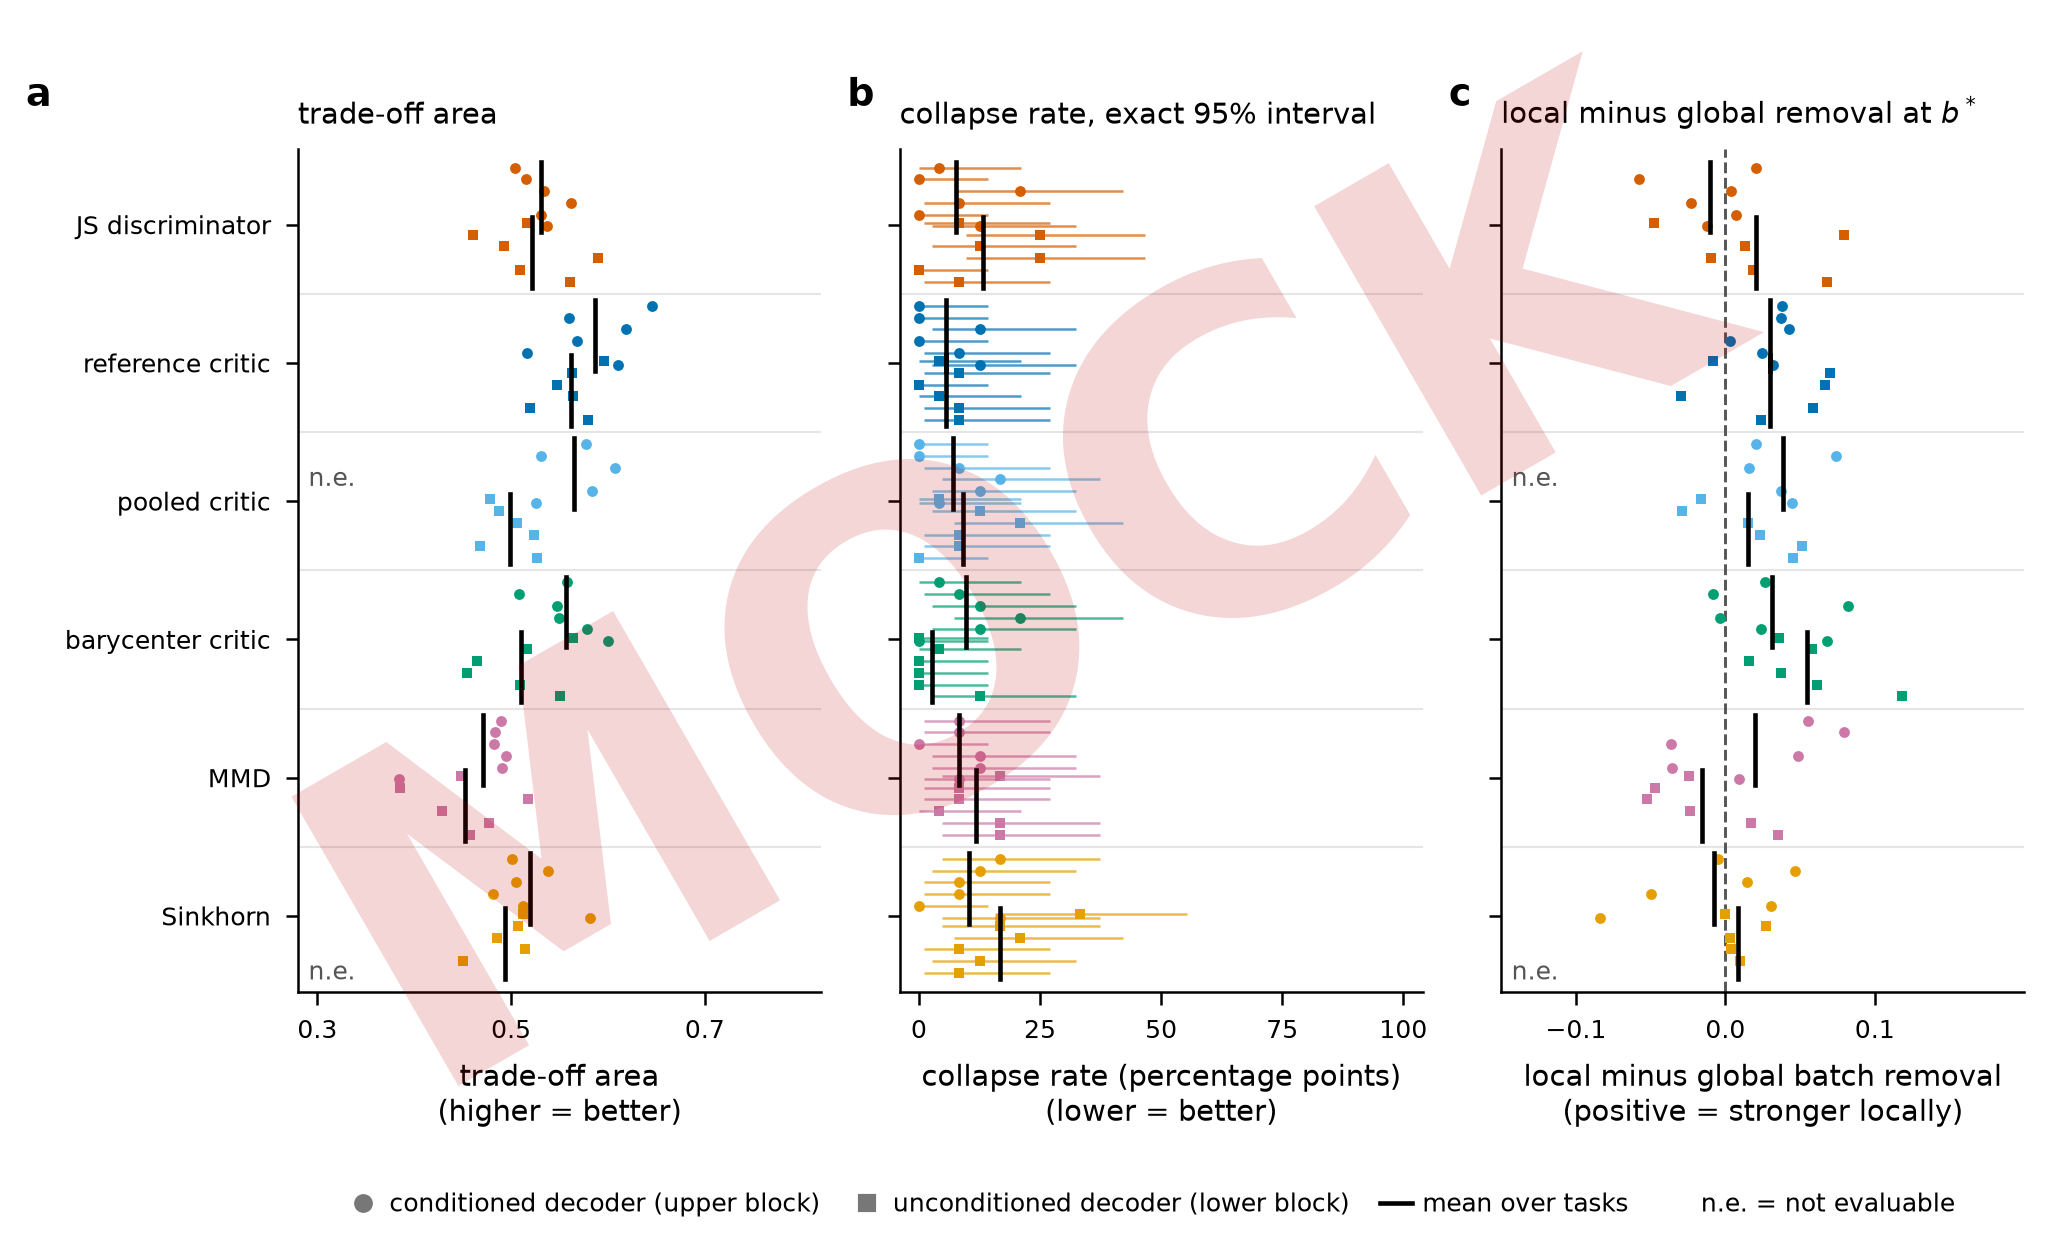
\includegraphics[width=\textwidth]{figures/mock/fig4.png}
\caption{\replaced{MOCK -- synthetic data. Secondary analyses per penalty, for the conditioned and unconditioned decoder. (a) Trade-off area; (b) collapse rate, percentage points, with exact 95\% intervals; (c) local minus global batch removal at $b^*$. One point per real task, tick is the mean; n.e., not evaluable.}{MOCK -- synthetic data. Reference critic minus discriminator, per real task and pooled over six real tasks, for each decoder. (a) Biology kept at matched batch removal $b^*$ (primary comparison); (b) trade-off area; (c) collapse rate, percentage points; (d) local minus global batch removal at $b^*$. Bars, 95\% intervals; grey band, margin below which a difference is not counted as real. n.e., not evaluable.}}
\label{fig:4}
\end{figure}

% ---------------------------------------------------------------- Figure 5
\begin{figure}[t]
\centering
% MOCK NEEDS REDRAW: single panel: width of each penalty's range of good strengths, in decades, one point per task and decoder; drop the old panel (b) follow-up variants.
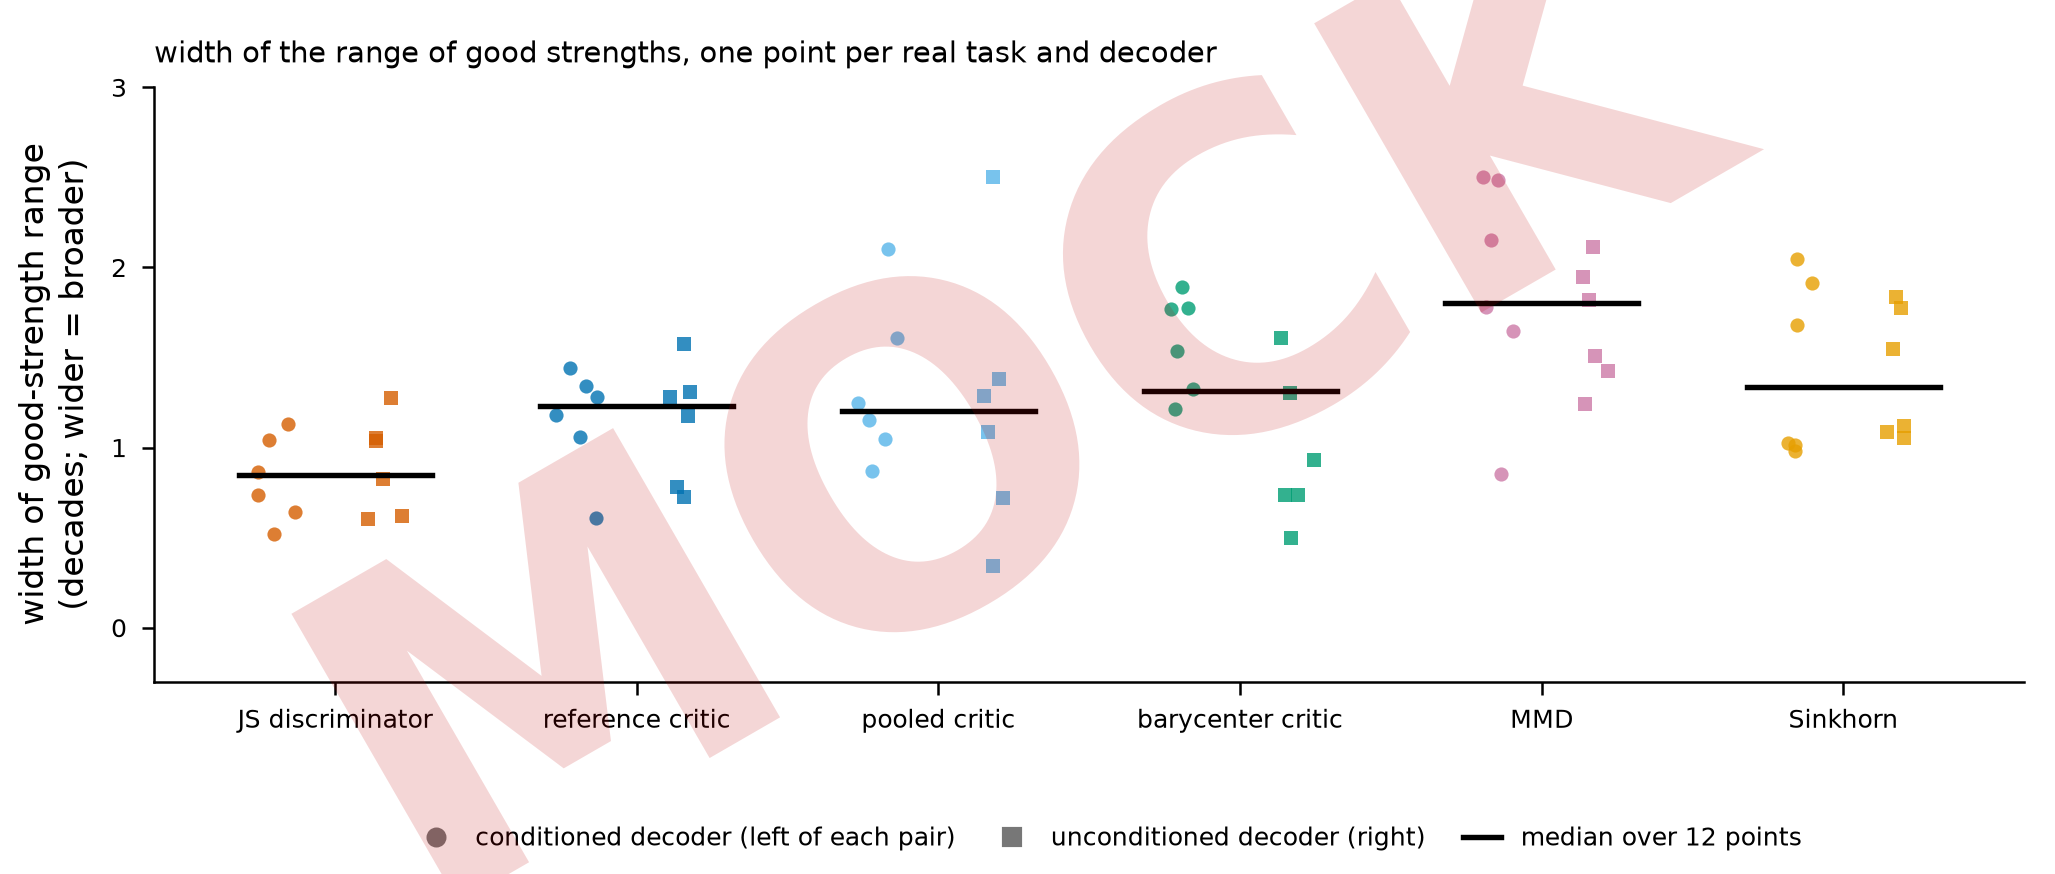
\includegraphics[width=\textwidth]{figures/mock/fig5.png}
\caption{\replaced{MOCK -- synthetic data. Width of each penalty's range of good strengths, in decades, one point per task and decoder; a good strength has a mean selection score at least the lower 95\% confidence bound of the best strength.}{MOCK -- synthetic data. (a) Width of each penalty's range of good strengths, in decades, one point per task and decoder; a good strength has a mean selection score at least the lower 95\% confidence bound of the best strength. (b) Follow-up experiment: biology at the matched strength, variant minus plain discriminator, with 95\% intervals. SN, spectral normalisation; GP, gradient penalty; starred rows, confirmatory contrast.}}
\label{fig:5}
\end{figure}

% ---------------------------------------------------------------- Figure 6
\begin{figure}[t]
\centering
% MOCK NEEDS REDRAW (pass 3): panel (a) shows the mean over the six real tasks of each method's per-task curve; per-task curves go in new Supplementary Figure S6. Figure 2: not-ranked hatching only for low-signal pairs (penalties not reaching b* take the bottom rank); mean over the real tasks that are not low-signal.
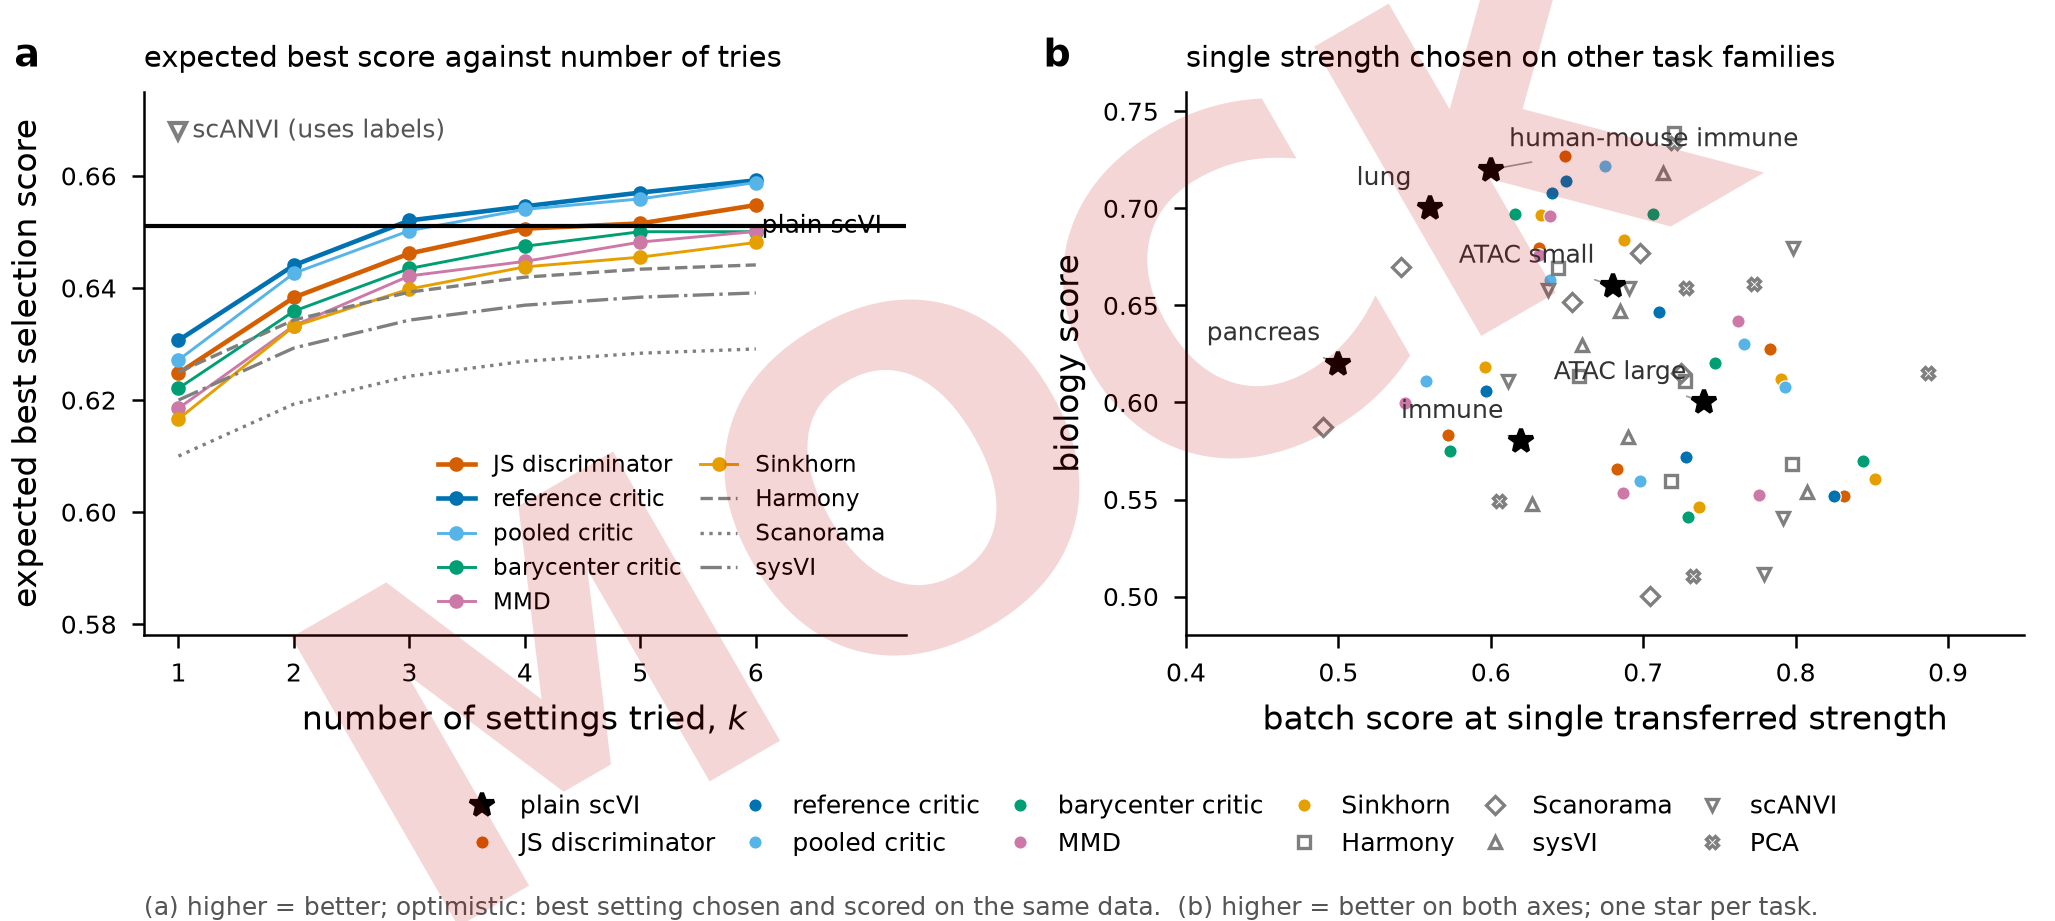
\includegraphics[width=\textwidth]{figures/mock/fig6.png}
\caption{MOCK -- synthetic data. Placement against plain scVI and standard tools. (a) Expected best selection score among $k$ settings drawn at random, $k=1$--6, \replaced[id=P3]{mean over the six real tasks of each method's per-task curve (Supplementary Figure S6)}{pooled over real tasks}, conditioned decoder; horizontal line, plain scVI; scANVI uses cell-type labels. (b) Batch against biology score per real task at the single strength chosen on other task families; stars, plain scVI; grey symbols, standard tools.}
\label{fig:6}
\end{figure}

% ---------------------------------------------------------------- Table 1
\begin{table}[t]
\centering\small
\caption{Alignment methods compared on the shared scVI backbone. Each penalty is multiplied by a fixed strength and added to the scVI loss. W1, Wasserstein-1; JS, Jensen--Shannon; MMD, maximum mean discrepancy; OT, optimal transport\added{; KL, Kullback--Leibler}. Equations in Supplementary Note 1; training settings in Supplementary Note 2 and Table S2.}
\label{tab:1}
\begin{tabular}{@{}>{\raggedright\arraybackslash}p{2.2cm}>{\raggedright\arraybackslash}p{4.5cm}>{\raggedright\arraybackslash}p{2.3cm}>{\centering\arraybackslash}p{1.5cm}>{\raggedright\arraybackslash}p{2.6cm}>{\raggedright\arraybackslash}p{2.8cm}@{}}
\toprule
Method & Alignment term & Network & Adversary steps per encoder step & Gradient penalty or regularisation & \replaced{Strength grid family (Table 2)}{Follow-up variants} \\
\midrule
JS discriminator & scvi-tools fool loss (JS-type): encoder trained to make the batch classifier wrong & batch classifier, two hidden layers of 128 units, one output per batch & 1 & none (plain) & \replaced{JS discriminator}{spectral normalisation; R1 gradient penalty; spectral normalisation + critic optimiser} \\
Reference critic & W1 distance of each batch to one reference batch (highest cell-type entropy) & critic, two hidden layers of 128 units, one output per batch & 5 & gradient penalty, weight 10 & \replaced{W1 critics (shared)}{none (the follow-up uses the pooled critic)} \\
Pooled critic & W1 distance of each batch to all other batches pooled & critic, as above & 5 & gradient penalty, weight 10 & \replaced{W1 critics (shared)}{gradient penalty at 1, 5 and 10 steps; spectral normalisation at 1 and 5 steps} \\
Barycenter critic & W1 distance of each batch to the minibatch Wasserstein barycenter (an average distribution) & critic, as above & 5 & gradient penalty, weight 10 & \replaced{W1 critics (shared)}{none} \\
MMD & kernel two-sample distance between batches, multi-scale Gaussian kernel & none & -- & none & \replaced{MMD}{none} \\
Sinkhorn & debiased Sinkhorn divergence (entropy-regularised OT); not W1 at this smoothing & none & -- & \replaced{entropic smoothing (Supplementary Table S2)}{entropic smoothing $0.05\sqrt{2d}$, $d$ the latent dimension} & \replaced{Sinkhorn divergence}{none} \\
scvi-tools adversary & scvi-tools adversarial batch classifier (reference method, conditioned decoder only) & batch classifier (scvi-tools default, two hidden layers of 32 units) & 1 & none; its weight is one minus the KL weight & \replaced{no strength grid}{none} \\
\bottomrule
\end{tabular}
\end{table}

% ---------------------------------------------------------------- Table 2 (provisional pilot ranges)
\begin{table}[t]
\centering\small
\caption{\added{Provisional, from the earlier three-task pilot; to be replaced.} Penalty strength ranges chosen in the strength pilot for each penalty family and decoder\deleted{ (three tasks, three seeds, ten strengths from 0.1 to 3,000 plus two further strengths where a range reached the grid edge)}. Each cell lists the six strengths fitted in the main benchmark, spread evenly on a log scale over the chosen range or, where that range held fewer than six half-decade values, with neighbouring values added above it first; the no-effect and over-correction ends of each range are in Supplementary Table S3 and the choice rules in Supplementary Note 4.}
\label{tab:2}
\begin{tabular}{@{}lll@{}}
\toprule
Penalty family (methods) & Conditioned decoder & Unconditioned decoder \\
\midrule
JS discriminator & 0.1, 0.3, 1, 3, 10, 30 & 0.03, 0.1, 0.3, 1, 3, 10 \\
W1 critics (reference, pooled, barycenter) & 0.1, 0.3, 3, 10, 100, 300 & 0.3, 1, 3, 10, 30, 100 \\
MMD & 3, 10, 30, 300, 1,000, 3,000 & 3, 10, 30, 100, 300, 1,000 \\
Sinkhorn divergence & 0.3, 3, 30, 100, 1,000, 10,000 & 0.3, 1, 3, 30, 100, 300 \\
\bottomrule
\end{tabular}
\end{table}

% ---------------------------------------------------------------- Table 3
\begin{table}[t]
\centering\small
\caption{\replaced{MOCK -- placeholder values. Benchmark ranking of the six penalties by biology score at matched batch removal $b^*$. Mean rank over the real tasks that are not low-signal (rank 1 is best; tied penalties share the average rank, and a penalty whose curve does not reach $b^*$ takes the bottom rank) and its range over tasks; mean biology score at $b^*$; ranks in simulation 1 and simulation 2, which are ranked separately; real tasks not ranked (low-signal) and number of real tasks ranked, of six. Per-task values are in Supplementary Table S6.}{MOCK -- placeholder values. Primary results, reference critic minus discriminator, pooled over the six real tasks. Estimate and 95\% posterior interval; posterior probabilities that the difference lies below $-m$, within $\pm m$, and above $m$ (margin $m=0.01$ for biology at $b^*$ and trade-off area, 5 percentage points for collapse rate); call (direction, practical equivalence or inconclusive); number of evaluable real tasks of six.}}
\label{tab:3}
\setlength{\tabcolsep}{3pt}
\begin{tabular}{@{}llrrrrrlc@{}}
\toprule
Penalty & Decoder & Mean rank & Range & Biology & Sim.\ 1 rank & Sim.\ 2 rank & Not ranked & Ranked \\
\midrule
JS discriminator & conditioned & xx.xx & [xx.xx, xx.xx] & x.xx & x.xx & x.xx & xx & x/6 \\
                  & unconditioned & xx.xx & [xx.xx, xx.xx] & x.xx & x.xx & x.xx & xx & x/6 \\
Reference critic & conditioned & xx.xx & [xx.xx, xx.xx] & x.xx & x.xx & x.xx & xx & x/6 \\
                  & unconditioned & xx.xx & [xx.xx, xx.xx] & x.xx & x.xx & x.xx & xx & x/6 \\
Pooled critic & conditioned & xx.xx & [xx.xx, xx.xx] & x.xx & x.xx & x.xx & xx & x/6 \\
                  & unconditioned & xx.xx & [xx.xx, xx.xx] & x.xx & x.xx & x.xx & xx & x/6 \\
Barycenter critic & conditioned & xx.xx & [xx.xx, xx.xx] & x.xx & x.xx & x.xx & xx & x/6 \\
                  & unconditioned & xx.xx & [xx.xx, xx.xx] & x.xx & x.xx & x.xx & xx & x/6 \\
MMD & conditioned & xx.xx & [xx.xx, xx.xx] & x.xx & x.xx & x.xx & xx & x/6 \\
                  & unconditioned & xx.xx & [xx.xx, xx.xx] & x.xx & x.xx & x.xx & xx & x/6 \\
Sinkhorn & conditioned & xx.xx & [xx.xx, xx.xx] & x.xx & x.xx & x.xx & xx & x/6 \\
                  & unconditioned & xx.xx & [xx.xx, xx.xx] & x.xx & x.xx & x.xx & xx & x/6 \\
\bottomrule
\end{tabular}
\end{table}

% ---------------------------------------------------------------- Table 4
\begin{table}[t]
\centering\small
\caption{MOCK -- placeholder values. Single-strength placement: mean selection score over five seeds ($0.4\times$batch $+\,0.6\times$biology) per method and real task, conditioned decoder, at the strength with the best mean selection score on real tasks of other families (related tasks never choose for each other). Values in parentheses use the task's own best strength (optimistic bound). \replaced[id=P3]{Harmony, Scanorama and sysVI are placed by the same rule, at the setting chosen on real tasks of other families, with the task's own best setting in parentheses; scANVI and principal-component analysis (PCA) run at one setting, so no choice is made; scANVI uses cell-type labels.}{Standard tools at their best setting; scANVI uses cell-type labels.} Unconditioned decoder in Supplementary Table \replaced{S7}{[to be decided: S-number]}.}
\label{tab:4}
\setlength{\tabcolsep}{3.5pt}
\begin{tabular}{@{}lcccccc@{}}
\toprule
Method & Pancreas & Lung & Immune & ATAC small & ATAC large & Human--mouse immune \\
\midrule
Plain scVI & xx.xx & xx.xx & xx.xx & xx.xx & xx.xx & xx.xx \\
scvi-tools adversary & xx.xx & xx.xx & xx.xx & xx.xx & xx.xx & xx.xx \\
JS discriminator & xx.xx (xx.xx) & xx.xx (xx.xx) & xx.xx (xx.xx) & xx.xx (xx.xx) & xx.xx (xx.xx) & xx.xx (xx.xx) \\
Reference critic & xx.xx (xx.xx) & xx.xx (xx.xx) & xx.xx (xx.xx) & xx.xx (xx.xx) & xx.xx (xx.xx) & xx.xx (xx.xx) \\
Pooled critic & xx.xx (xx.xx) & xx.xx (xx.xx) & xx.xx (xx.xx) & xx.xx (xx.xx) & xx.xx (xx.xx) & xx.xx (xx.xx) \\
Barycenter critic & xx.xx (xx.xx) & xx.xx (xx.xx) & xx.xx (xx.xx) & xx.xx (xx.xx) & xx.xx (xx.xx) & xx.xx (xx.xx) \\
MMD & xx.xx (xx.xx) & xx.xx (xx.xx) & xx.xx (xx.xx) & xx.xx (xx.xx) & xx.xx (xx.xx) & xx.xx (xx.xx) \\
Sinkhorn & xx.xx (xx.xx) & xx.xx (xx.xx) & xx.xx (xx.xx) & xx.xx (xx.xx) & xx.xx (xx.xx) & xx.xx (xx.xx) \\
\midrule
Harmony & xx.xx (xx.xx) & xx.xx (xx.xx) & xx.xx (xx.xx) & xx.xx (xx.xx) & xx.xx (xx.xx) & xx.xx (xx.xx) \\
Scanorama & xx.xx (xx.xx) & xx.xx (xx.xx) & xx.xx (xx.xx) & xx.xx (xx.xx) & xx.xx (xx.xx) & xx.xx (xx.xx) \\
sysVI & xx.xx (xx.xx) & xx.xx (xx.xx) & xx.xx (xx.xx) & xx.xx (xx.xx) & xx.xx (xx.xx) & xx.xx (xx.xx) \\
scANVI (labels) & xx.xx & xx.xx & xx.xx & xx.xx & xx.xx & xx.xx \\
PCA (uncorrected) & xx.xx & xx.xx & xx.xx & xx.xx & xx.xx & xx.xx \\
\bottomrule
\end{tabular}
\end{table}
\clearpage
\vspace{4pt}
\begin{multicols}{2}
\renewcommand{\refname}{References}
\bibliographystyle{plainnat}
\bibliography{refs}
\end{multicols}
\end{document}
